% Options for packages loaded elsewhere
\PassOptionsToPackage{unicode}{hyperref}
\PassOptionsToPackage{hyphens}{url}
\PassOptionsToPackage{dvipsnames,svgnames,x11names}{xcolor}
%
\documentclass[
  letterpaper,
  DIV=11,
  numbers=noendperiod]{scrartcl}

\usepackage{amsmath,amssymb}
\usepackage{setspace}
\usepackage{iftex}
\ifPDFTeX
  \usepackage[T1]{fontenc}
  \usepackage[utf8]{inputenc}
  \usepackage{textcomp} % provide euro and other symbols
\else % if luatex or xetex
  \usepackage{unicode-math}
  \defaultfontfeatures{Scale=MatchLowercase}
  \defaultfontfeatures[\rmfamily]{Ligatures=TeX,Scale=1}
\fi
\usepackage{lmodern}
\ifPDFTeX\else  
    % xetex/luatex font selection
\fi
% Use upquote if available, for straight quotes in verbatim environments
\IfFileExists{upquote.sty}{\usepackage{upquote}}{}
\IfFileExists{microtype.sty}{% use microtype if available
  \usepackage[]{microtype}
  \UseMicrotypeSet[protrusion]{basicmath} % disable protrusion for tt fonts
}{}
\makeatletter
\@ifundefined{KOMAClassName}{% if non-KOMA class
  \IfFileExists{parskip.sty}{%
    \usepackage{parskip}
  }{% else
    \setlength{\parindent}{0pt}
    \setlength{\parskip}{6pt plus 2pt minus 1pt}}
}{% if KOMA class
  \KOMAoptions{parskip=half}}
\makeatother
\usepackage{xcolor}
\usepackage[left=2.54cm,right=2.54cm,top=2.54cm,bottom=2.54cm]{geometry}
\setlength{\emergencystretch}{3em} % prevent overfull lines
\setcounter{secnumdepth}{-\maxdimen} % remove section numbering
% Make \paragraph and \subparagraph free-standing
\makeatletter
\ifx\paragraph\undefined\else
  \let\oldparagraph\paragraph
  \renewcommand{\paragraph}{
    \@ifstar
      \xxxParagraphStar
      \xxxParagraphNoStar
  }
  \newcommand{\xxxParagraphStar}[1]{\oldparagraph*{#1}\mbox{}}
  \newcommand{\xxxParagraphNoStar}[1]{\oldparagraph{#1}\mbox{}}
\fi
\ifx\subparagraph\undefined\else
  \let\oldsubparagraph\subparagraph
  \renewcommand{\subparagraph}{
    \@ifstar
      \xxxSubParagraphStar
      \xxxSubParagraphNoStar
  }
  \newcommand{\xxxSubParagraphStar}[1]{\oldsubparagraph*{#1}\mbox{}}
  \newcommand{\xxxSubParagraphNoStar}[1]{\oldsubparagraph{#1}\mbox{}}
\fi
\makeatother


\providecommand{\tightlist}{%
  \setlength{\itemsep}{0pt}\setlength{\parskip}{0pt}}\usepackage{longtable,booktabs,array}
\usepackage{calc} % for calculating minipage widths
% Correct order of tables after \paragraph or \subparagraph
\usepackage{etoolbox}
\makeatletter
\patchcmd\longtable{\par}{\if@noskipsec\mbox{}\fi\par}{}{}
\makeatother
% Allow footnotes in longtable head/foot
\IfFileExists{footnotehyper.sty}{\usepackage{footnotehyper}}{\usepackage{footnote}}
\makesavenoteenv{longtable}
\usepackage{graphicx}
\makeatletter
\newsavebox\pandoc@box
\newcommand*\pandocbounded[1]{% scales image to fit in text height/width
  \sbox\pandoc@box{#1}%
  \Gscale@div\@tempa{\textheight}{\dimexpr\ht\pandoc@box+\dp\pandoc@box\relax}%
  \Gscale@div\@tempb{\linewidth}{\wd\pandoc@box}%
  \ifdim\@tempb\p@<\@tempa\p@\let\@tempa\@tempb\fi% select the smaller of both
  \ifdim\@tempa\p@<\p@\scalebox{\@tempa}{\usebox\pandoc@box}%
  \else\usebox{\pandoc@box}%
  \fi%
}
% Set default figure placement to htbp
\def\fps@figure{htbp}
\makeatother
% definitions for citeproc citations
\NewDocumentCommand\citeproctext{}{}
\NewDocumentCommand\citeproc{mm}{%
  \begingroup\def\citeproctext{#2}\cite{#1}\endgroup}
\makeatletter
 % allow citations to break across lines
 \let\@cite@ofmt\@firstofone
 % avoid brackets around text for \cite:
 \def\@biblabel#1{}
 \def\@cite#1#2{{#1\if@tempswa , #2\fi}}
\makeatother
\newlength{\cslhangindent}
\setlength{\cslhangindent}{1.5em}
\newlength{\csllabelwidth}
\setlength{\csllabelwidth}{3em}
\newenvironment{CSLReferences}[2] % #1 hanging-indent, #2 entry-spacing
 {\begin{list}{}{%
  \setlength{\itemindent}{0pt}
  \setlength{\leftmargin}{0pt}
  \setlength{\parsep}{0pt}
  % turn on hanging indent if param 1 is 1
  \ifodd #1
   \setlength{\leftmargin}{\cslhangindent}
   \setlength{\itemindent}{-1\cslhangindent}
  \fi
  % set entry spacing
  \setlength{\itemsep}{#2\baselineskip}}}
 {\end{list}}
\usepackage{calc}
\newcommand{\CSLBlock}[1]{\hfill\break\parbox[t]{\linewidth}{\strut\ignorespaces#1\strut}}
\newcommand{\CSLLeftMargin}[1]{\parbox[t]{\csllabelwidth}{\strut#1\strut}}
\newcommand{\CSLRightInline}[1]{\parbox[t]{\linewidth - \csllabelwidth}{\strut#1\strut}}
\newcommand{\CSLIndent}[1]{\hspace{\cslhangindent}#1}

\usepackage{booktabs}
\usepackage{longtable}
\usepackage{array}
\usepackage{multirow}
\usepackage{wrapfig}
\usepackage{float}
\usepackage{colortbl}
\usepackage{pdflscape}
\usepackage{tabu}
\usepackage{threeparttable}
\usepackage{threeparttablex}
\usepackage[normalem]{ulem}
\usepackage{makecell}
\usepackage{xcolor}
\KOMAoption{captions}{tableheading}
\makeatletter
\@ifpackageloaded{caption}{}{\usepackage{caption}}
\AtBeginDocument{%
\ifdefined\contentsname
  \renewcommand*\contentsname{Tabla de contenidos}
\else
  \newcommand\contentsname{Tabla de contenidos}
\fi
\ifdefined\listfigurename
  \renewcommand*\listfigurename{Listado de Figuras}
\else
  \newcommand\listfigurename{Listado de Figuras}
\fi
\ifdefined\listtablename
  \renewcommand*\listtablename{Listado de Tablas}
\else
  \newcommand\listtablename{Listado de Tablas}
\fi
\ifdefined\figurename
  \renewcommand*\figurename{Figura}
\else
  \newcommand\figurename{Figura}
\fi
\ifdefined\tablename
  \renewcommand*\tablename{Tabla}
\else
  \newcommand\tablename{Tabla}
\fi
}
\@ifpackageloaded{float}{}{\usepackage{float}}
\floatstyle{ruled}
\@ifundefined{c@chapter}{\newfloat{codelisting}{h}{lop}}{\newfloat{codelisting}{h}{lop}[chapter]}
\floatname{codelisting}{Listado}
\newcommand*\listoflistings{\listof{codelisting}{Listado de Listados}}
\makeatother
\makeatletter
\makeatother
\makeatletter
\@ifpackageloaded{caption}{}{\usepackage{caption}}
\@ifpackageloaded{subcaption}{}{\usepackage{subcaption}}
\makeatother

\ifLuaTeX
\usepackage[bidi=basic]{babel}
\else
\usepackage[bidi=default]{babel}
\fi
\babelprovide[main,import]{spanish}
% get rid of language-specific shorthands (see #6817):
\let\LanguageShortHands\languageshorthands
\def\languageshorthands#1{}
\usepackage{bookmark}

\IfFileExists{xurl.sty}{\usepackage{xurl}}{} % add URL line breaks if available
\urlstyle{same} % disable monospaced font for URLs
\hypersetup{
  pdftitle={Perfiles de Individualismo en la sociedad chilena},
  pdfauthor={Gabriel Cortés Paredes},
  pdflang={es},
  pdfkeywords={Individualismo, Individuación, Análisis de clases
latentes},
  colorlinks=true,
  linkcolor={blue},
  filecolor={Maroon},
  citecolor={Blue},
  urlcolor={Blue},
  pdfcreator={LaTeX via pandoc}}


\title{Perfiles de Individualismo en la sociedad chilena}
\author{Gabriel Cortés Paredes}
\date{}

\begin{document}
\maketitle
\begin{abstract}
Escribir
\end{abstract}


\setstretch{1.15}
\section*{Antecedentes}\label{antecedentes}
\addcontentsline{toc}{section}{Antecedentes}

El presente trabajo busca explorar la relación entre los perfiles de
individualismo y el apoyo a un líder fuerte en la sociedad chilena. En
un contexto político que, tanto a nivel nacional como internacional, los
liderazgos autoritarios y populistas cobran mayor relevancia, esta
investigación se centra en entender como divergencias en los procesos de
individuación pueden estar asociados con formas de ejercer el poder que
se alejan del ideal democrático y representativo. De tal modo, esta
investigación se propone arrojar luz sobre las consecuencias políticas
del individualismo, en sus distintas expresiones, en la sociedad
chilena.

En los últimos años ha sido posible observar varios indicadores que
apuntan hacia una disminución en el apoyo de los chilenos a la
democracia (\citeproc{ref-cep}{CEP 2023}), sumado a un aumento en las
preferencias por opciones populistas o autoritarias
(\citeproc{ref-cadem2023}{CADEM 2023};
\citeproc{ref-cerc-mori}{CERC-MORI 2023}; \citeproc{ref-diaz2023}{Díaz,
Rovira Kaltwasser, y Zanotti 2023}), así como un profundo
distanciamiento entre élites políticas y la ciudadanía
(\citeproc{ref-luna2016}{Luna 2016}). En este contexto, resulta
plausible que surjan tendencias que aboguen por liderazgos fuertes
capaces de cumplir con eficacia las demandas de los ciudadanos, incluso
a expensas de respaldar soluciones autoritarias o no-democráticas
(\citeproc{ref-carlin2018}{Carlin 2018}).

Por supuesto, la disminución del apoyo a la democracia y el surgimiento
de opciones autoritarias o populistas no es un fenómeno únicamente
local, y ha sido estudiado ampliamente en varias regiones del mundo bajo
diversas etiquetas, tales como \emph{liderazgos fuertes, no-democráticos
o delegativos} (\citeproc{ref-carlin2011}{Carlin 2011},
\citeproc{ref-carlin2018}{2018}; \citeproc{ref-crimston2022}{Crimston,
Selvanathan, y Jetten 2022}; \citeproc{ref-kang2018}{Kang y Lee 2018};
\citeproc{ref-lima2021}{Lima et~al. 2021};
\citeproc{ref-selvanathan2022}{Selvanathan, Crimston, y Jetten 2022};
\citeproc{ref-xuereb2021}{Xuereb et~al. 2021}), \emph{populismos}
(\citeproc{ref-baro2022}{Baro 2022}; \citeproc{ref-gidron2020}{Gidron y
Hall 2020}; \citeproc{ref-nowakowski2021}{Nowakowski 2021}), o
\emph{derecha populista radical} (\citeproc{ref-diaz2023}{Díaz, Rovira
Kaltwasser, y Zanotti 2023}; \citeproc{ref-donovan2019}{Donovan 2019},
\citeproc{ref-donovan2021}{2021}). También se han puesto esfuerzos en
identificar sus determinantes, entre los que se pueden contar factores
culturales (\citeproc{ref-lima2021}{Lima et~al. 2021};
\citeproc{ref-marchlewska2022}{Marchlewska et~al. 2022};
\citeproc{ref-selvanathan2022}{Selvanathan, Crimston, y Jetten 2022});
factores económicos objetivos y subjetivos
(\citeproc{ref-arikan2019}{Arikan y Sekercioglu 2019};
\citeproc{ref-rico2020}{Rico, Guinjoan, y Anduiza 2020};
\citeproc{ref-wu2019}{Wu y Chang 2019}; \citeproc{ref-xuereb2021}{Xuereb
et~al. 2021}); el bajo bienestar o estatus subjetivo
(\citeproc{ref-gidron2020}{Gidron y Hall 2020};
\citeproc{ref-nowakowski2021}{Nowakowski 2021}); sentimientos de anomia
y de polarización moral (\citeproc{ref-crimston2022}{Crimston,
Selvanathan, y Jetten 2022}); la pertenencia a una minoría étnica o
religiosa con baja integración nacional
(\citeproc{ref-eskelinen2020}{Eskelinen y Verkuyten 2020}); así como
rasgos personales como el narcisismo
(\citeproc{ref-marchlewska2019}{Marchlewska et~al. 2019}), la
autoeficacia (\citeproc{ref-rico2020}{Rico, Guinjoan, y Anduiza 2020}) o
el privilegiar los valores de conservación (\citeproc{ref-baro2022}{Baro
2022}).

En este contexto, es relevante destacar que existen algunos estudios que
han explorado la relación entre distintos modelos de democracia,
preferencias o actitudes políticas y el espectro
Individualismo-Colectivismo. Bajo el enfoque popularizado por Geert
Hofstede en la década de 1980, Individualismo y Colectivismo representan
dos extremos de un continúo que permite diferenciar entre diversas
culturas (\citeproc{ref-oyserman2002}{Oyserman, Coon, y Kemmelmeier
2002}). En sociedades individualistas, se espera que los individuos
asuman la responsabilidad de sus propias vidas y las de sus familias,
mientras que las culturas colectivistas se caracterizan por la
existencia de sólidos lazos de interdependencia entre sus miembros
(\citeproc{ref-yoon2010}{Yoon 2010}).

Bajo este enfoque, se ha observado que, entre estudiantes universitarios
estadounidenses, el individualismo y el colectivismo son dimensiones
ortogonales, con el primero ubicado en el polo opuesto al autoritarismo
(\citeproc{ref-gelfand1996}{Gelfand, Triandis, y Chan 1996}). Por otro
lado, en una serie de estudios comparativos realizados en varios países,
estos hallazgos se han complejizado al encontrar una asociación positiva
entre el autoritarismo y el individualismo vertical, que privilegia la
competencia y la jerarquía entre individuos, pero no con el
individualismo horizontal, que fomenta la unicidad y la igualdad
(\citeproc{ref-kemmelmeier2003}{Kemmelmeier et~al. 2003}). Asimismo, se
ha observado que el individualismo vertical está relacionado con
orientaciones de dominancia social (\citeproc{ref-strunk1999}{Strunk y
Chang 1999}) y con el voto conservador en los Estados Unidos
(\citeproc{ref-zhang2009}{Zhang, Nelson, y Mao 2009}). Además, se ha
argumentado que las culturas individualistas promueven una mejor
gobernanza al desincentivar la corrupción, el nepotismo y el
clientelismo (\citeproc{ref-kyriacou2016}{Kyriacou 2016}).

Sin embargo, estos estudios son escasos y comparten ciertas
limitaciones. Estas investigaciones suelen restringir las definiciones
de individualismo y colectivismo a un nivel puramente cultural, sin
adentrarse en el análisis de posibles divergencias dentro de una misma
sociedad. Además, ninguno de estos estudios ha explorado estos fenómenos
en el contexto chileno o en América Latina.

De tal modo, considerando las consecuencias políticas
(\citeproc{ref-zhang2009}{Zhang, Nelson, y Mao 2009}), sociales
(\citeproc{ref-strunk1999}{Strunk y Chang 1999}) y económicas
(\citeproc{ref-kyriacou2016}{Kyriacou 2016}) que se derivan de la
asociación entre el individualismo y las actitudes o preferencias
políticas, se plantea la necesidad de emprender una investigación que
aborde las brechas antes mencionadas. Para lograrlo, y como se
argumentará en detalle más adelante, se incluirá un giro en la
conceptualización de individualismo, que busca pasar a entenderlo como
el resultado de procesos sociohistóricos de individuación que difieren
no solo entre culturas, sino también dentro de una misma sociedad
(\citeproc{ref-martuccelli2018}{Martuccelli 2018}).

La individuación es un fenómeno sociohistórico que provoca cambios en la
manera en que los individuos se relacionan con las figuras de autoridad
(\citeproc{ref-araujo2021}{Araujo 2021}). Por ello, parece interesante
indagar cómo diferentes variantes de individualismo -- resultado de
divergencias de los procesos de individuación -- podrían relacionarse
con la pérdida de legitimidad de modalidades democráticas de autoridad,
privilegiando, por ejemplo, liderazgos percibidos como más fuertes,
eficientes (\citeproc{ref-araujo2022}{Araujo et~al. 2022};
\citeproc{ref-araujo2022a}{Araujo 2022}), o auténticos
(\citeproc{ref-gauthier2021}{Gauthier 2021}). En visto de todo lo
planteado, este artículo se propone como objetivo el establecer la
relación entre el apoyo a un líder fuerte y los distintos perfiles de
individualismo en la sociedad chilena.

A continuación, se presentará un marco teórico donde se definirán ambos
conceptos centrales de esta investigación. Luego, se expondrá la
estrategia metodológica propuesta, que incluirá la presentación de la
muestra, los indicadores y las técnicas de análisis utilizadas.
Posteriormente, se procederá a mostrar los principales hallazgos del
estudio, identificando los perfiles de individualismo y estableciendo su
relación con el apoyo a un líder fuerte. Estos resultados serán luego
discutidos a la luz del modelo teórico presentado. Finalmente, el
documento cerrará con algunas reflexiones sobre las limitaciones de esta
investigación, así como con las perspectivas que deja abiertas.

\section*{Marco Teórico}\label{marco-teuxf3rico}
\addcontentsline{toc}{section}{Marco Teórico}

\subsection*{Apoyo a un Líder Fuerte}\label{apoyo-a-un-luxedder-fuerte}
\addcontentsline{toc}{subsection}{Apoyo a un Líder Fuerte}

Se entenderá el apoyo a un Líder Fuerte como la demanda, por parte de
los ciudadanos, de que el poder político esté concentrado en un líder,
ejerciéndolo de manera personalista, con poco o nulo contrapeso por
parte de otras instituciones o actores. Pese a que este tipo de
liderazgos se han considerado como más comunes en regímenes autoritarios
(\citeproc{ref-kendall-taylor2017}{Kendall-Taylor, Frantz, y Wright
2017}), durante las últimas décadas se ha observado su auge también en
democracias liberales consolidadas
(\citeproc{ref-lindstaedt2021}{Lindstaedt 2021};
\citeproc{ref-kendall-taylor2017}{Kendall-Taylor, Frantz, y Wright
2017}).

Se ha propuesto que este tipo de liderazgo tiene mayores posibilidades
de aparecer en contextos negativos o de incertidumbre, donde un líder
fuerte suele ser percibido como una solución a problemas políticos o
económicos (\citeproc{ref-harms2018}{Harms et~al. 2018}). El ascenso al
poder de este tipo de líderes se ha asociado a una mayor polarización,
así como de procesos de concentración del poder y de deterioro
democrático (\citeproc{ref-lindstaedt2021}{Lindstaedt 2021};
\citeproc{ref-brunkert2023}{Brunkert y Von Soest 2023};
\citeproc{ref-kendall-taylor2017}{Kendall-Taylor, Frantz, y Wright
2017}). Pese a ello, el apoyo a este tipo de liderazgo ha crecido a lo
largo del mundo, y una parte importante de la literatura se ha dedicado
a comprender los factores de esta tendencia. Entre algunas explicaciones
que se han esbozado se cuentan rasgos de la personalidad como la
mentalidad cerrada o la introversión
(\citeproc{ref-armendarizmiranda2021}{Armendariz Miranda y Cawvey
2021}), la incertidumbre identitaria (\citeproc{ref-hogg2021}{Hogg
2021}; \citeproc{ref-hogg2013}{Hogg y Adelman 2013}), el deseo por
continuar la identidad nacional
(\citeproc{ref-selvanathan2022}{Selvanathan, Crimston, y Jetten 2022}),
la desigualdad económica (\citeproc{ref-sprong2019}{Sprong et~al. 2019})
y la baja confianza interpersonal (\citeproc{ref-xuereb2021}{Xuereb
et~al. 2021}).

Además, se ha indicado que el apoyo a un líder fuerte se encuentra
asociado a la llamada personalidad autoritaria
(\citeproc{ref-harms2018}{Harms et~al. 2018}). Particularmente, los
autoritarios estarían más dispuestos a renunciar a su autonomía personal
frente a autoridades percibidas como dominantes
(\citeproc{ref-harms2018}{Harms et~al. 2018}). En la misma línea, se ha
planteado que el individualismo no es tanto el opuesto al colectivismo,
sino del autoritarismo (\citeproc{ref-gelfand1996}{Gelfand, Triandis, y
Chan 1996}). De tal modo, existe una tendencia en la literatura a
asociar negativamente al individualismo con actitudes autoritarias,
planteando más bien una relación con el apoyo a las variantes más
liberales y representativas de democracia. Pese a ello, también se ha
encontrado evidencia empírica que apunta a la asociación entre el
individualismo con el conservadurismo (\citeproc{ref-zhang2009}{Zhang,
Nelson, y Mao 2009}), el autoritarismo
(\citeproc{ref-kemmelmeier2003}{Kemmelmeier et~al. 2003}) y la
dominancia social (\citeproc{ref-strunk1999}{Strunk y Chang 1999}). De
tal modo, el panorama general sugiere que la relación entre
individualismo y democracia está lejos de ser unívoca.

Frente a lo anterior, en la siguiente sección se presentará la propuesta
teórica de esta investigación. La apuesta aquí es que la sociología del
individuo entregaría las herramientas necesarias para comprender las
relaciones divergentes entre el individualismo y los tipos de liderazgos
demandados por la ciudadanía.

\subsection*{Individualismo}\label{individualismo}
\addcontentsline{toc}{subsection}{Individualismo}

El fenómeno del individualismo ha sido principalmente investigado desde
la psicología cultural, con un enfoque especial en la comparación entre
distintas culturas. Desde esta perspectiva, de tal modo, se tienden a
categorizar sociedades y países ya sea como individualistas o como
colectivistas. Las sociedades individualistas se caracterizarían por
lazos poco estrechos entre individuos, de quienes se espera se hagan
cargo de sí mismos y de su familia inmediata. Las sociedades
colectivistas, en tanto, se definen porque sus miembros están integrados
desde su nacimiento a grupos fuertemente cohesionados que los protegen a
lo largo de sus vidas a cambio de una lealtad incuestionable
(\citeproc{ref-yoon2010}{Yoon 2010}).

Esta conceptualización de individualismo-colectivismo ha sido criticada
por su falta de claridad conceptual
(\citeproc{ref-oyserman2002}{Oyserman, Coon, y Kemmelmeier 2002}), su
uso como un concepto \emph{catch-all}, que se utiliza por defecto para
explicar diferencias culturales (\citeproc{ref-voronov2002}{Voronov y
Singer 2002}) y que esconde una dimensión normativa que asocia el
individualismo a la modernidad y al desarrollo
(\citeproc{ref-voronov2002}{Voronov y Singer 2002};
\citeproc{ref-wang2010}{Wang y Liu 2010};
\citeproc{ref-martuccelli2010}{Martuccelli 2010};
\citeproc{ref-moemeka1998}{Moemeka 1998}). Brewer y Chen
(\citeproc{ref-brewer2007}{2007}) además, indican que no hay una
verdadera simetría en la forma en que se operacionalizan el
individualismo y el colectivismo, pues, mientras que los ítems
utilizados para medir el individualismo suelen centrarse en la identidad
y la agencia de los individuos, el colectivismo se suele medir como un
sistema de valores.

Estas limitaciones se expresan en ``anomalías'' observables en varios de
estos estudios, como que los individualistas pueden ser tanto o más
colectivistas que los colectivistas mismos
(\citeproc{ref-oyserman2002}{Oyserman, Coon, y Kemmelmeier 2002}), o que
en determinados contextos los colectivistas actúan de manera
individualista (\citeproc{ref-voronov2002}{Voronov y Singer 2002}). A
nivel agregado, Chile podría considerarse como un claro ejemplo de estas
contradicciones: Bajo la definición de Hofstede, la sociedad chilena ha
sido clasificada como colectivista
(\citeproc{ref-rojas2008}{Rojas-Méndez et~al. 2008}). Esto concuerda con
observaciones que han señalado que el colectivismo en Chile es alto,
tanto si se mide como el opuesto al individualismo
(\citeproc{ref-oyserman2002}{Oyserman, Coon, y Kemmelmeier 2002}) o
entendido como un \emph{self-construal} interdependiente
(\citeproc{ref-benavides2020}{Benavides y Hur 2020}). No obstante,
también es cierto que los niveles de individualismo observados en el
país llegan a ser incluso más altos que aquellos obtenidos en sociedades
típicamente individualistas, como Estados Unidos
(\citeproc{ref-oyserman2002}{Oyserman, Coon, y Kemmelmeier 2002}) o
Noruega (\citeproc{ref-kolstad2009}{Kolstad y Horpestad 2009}).

Esto abre la pregunta de si Chile realmente es una sociedad
colectivista, y si no lo es, ¿hasta qué punto es una sociedad
individualista? La propuesta de esta investigación es que, con el fin de
responder esta pregunta, es necesario dar un giro hacia una perspectiva
teórica que provea el lenguaje para describir el individualismo chileno.
En concreto, se conceptualizará el individualismo desde la sociología
del individuo desarrollada por Danilo Martuccelli. Desde este enfoque,
tanto en su obra individual (\citeproc{ref-martuccelli2010}{Martuccelli
2010}, \citeproc{ref-martuccelli2018}{2018}), como en colaboración con
Kathya Araujo (\citeproc{ref-araujo2014}{Araujo y Martuccelli 2014},
\citeproc{ref-araujo2020}{2020a}, \citeproc{ref-araujo2012}{2012}),
Martuccelli ha hecho esfuerzos contundentes para describir la forma
particular del individualismo en Chile y América Latina.

Martuccelli (\citeproc{ref-martuccelli2010}{2010}) argumenta que la
representación del individuo que se volvió hegemónica para la modernidad
es un individuo que es soberano en al menos dos acepciones. En primer
lugar, porque se espera de este que sea dueño de sí mismo, de manera
independiente, autónoma y singular. En segundo lugar, porque es un ente
racional capaz de legitimar el orden social y la soberanía colectiva.

Este individuo se encuentra en el vértice de un modelo de representación
de la vida social que lo sitúa en el centro del pacto social
(\citeproc{ref-martuccelli2010}{Martuccelli 2010},
\citeproc{ref-martuccelli2018}{2018}). Este modelo es lo que comúnmente
se entiende como individualismo. Martuccelli
(\citeproc{ref-martuccelli2018}{2018}) denomina a esta variante del
fenómeno como \emph{individualismo institucional}, caracterizado por una
separación radical entre holismo e individualismo, una concepción
atomizada del individuo y la preminencia del rol de las instituciones en
los procesos de individuación.

Las divergencias respecto a este modelo, observadas en otras regiones
del mundo, a menudo ha llevado de la negación existencia de individuos,
individualización e individualismo en éstas
(\citeproc{ref-martuccelli2010}{Martuccelli 2010}). En cambio, abordar
el fenómeno del individualismo desde la sociología del individuo permite
desembarazarse de estas conceptualizaciones unívocas. Frente a ello, se
propone una definición que permita teorizar el fenómeno para la sociedad
chilena.

Se entenderá así como individualismo a los modelos de representación de
la vida social que definen el rol del individuo en la sociedad. Bajo
tales modelos, los individuos deben hacerse cargo de sus propias vidas
en condiciones diversas de a) legitimidad de la acción individual, b)
distintas representaciones culturales y autoconcepciones del individuo,
y c) diferentes valores e imperativos estructuralmente producidos.

\textbf{La legitimidad de la acción individual} hace referencia a las
creencias sobre la agencia de los individuos en el mundo social
(\citeproc{ref-brewer2007}{Brewer y Chen 2007}) y la legitimidad de
acciones individualizadas en las esferas de la economía, la política y
las emociones (\citeproc{ref-cortois2018}{Cortois y Laermans 2018}). Una
mayor legitimidad de la acción individual se relaciona a una mayor
valoración de la individualidad, la cual se define como el ``grado de
diferenciación o de singularización reconocido o legítimamente alcanzado
por un individuo dentro de un colectivo''
(\citeproc{ref-martuccelli2018}{Martuccelli 2018, 10}).

Bajo el modelo del individualismo institucional, la individualidad deja
de ser una anomalía para pasar a ostentar altos niveles de legitimidad
(\citeproc{ref-martuccelli2018}{Martuccelli 2018}). Sin embargo, esto se
vería tensionado, por ejemplo, por la acentuación de conductas
individualizadas sin ruptura de lazos comunitarios en sociedades
africanas, modelo que Martuccelli (\citeproc{ref-martuccelli2018}{2018})
denomina como individualismo comunitario. Más cercano a la realidad
nacional, Araujo y Martuccelli (\citeproc{ref-araujo2020a}{2020b})
constatan que la individualidad ha sido históricamente vista con
sospecha en sociedades latinoamericanas.

Ahora bien, se debe resaltar que el individualismo ha sido
institucionalizado principalmente en 3 esferas: la económica, la
política y la afectiva (\citeproc{ref-cortois2018}{Cortois y Laermans
2018}; \citeproc{ref-martuccelli2018}{Martuccelli 2018}). Esto se
refleja en la existencia de 3 guiones para el individualismo
institucional; en la esfera económica, un individualismo utilitario que
legitima la acción individual estratégica, poniendo medio sobre fines;
en la política, un individualismo moral que enfatiza la obligación de
tratar al otro como un fin en sí mismo; y en la afectiva, un
individualismo expresivo en que la acción social se entiende como un
medio para la expresión auténtica del yo
(\citeproc{ref-cortois2018}{Cortois y Laermans 2018}).

\textbf{Las autoconcepciones del individuo}, por otro lado, abordan las
diversas concepciones en torno a las que se pueden definir las
identidades de los individuos en relación a sus grupos de referencia
(\citeproc{ref-brewer2007}{Brewer y Chen 2007}).

La concepción independiente es aquella en que el individuo se concibe
como un ente atomizado y prexistente a sus lazos sociales. Aunque esta
concepción se ha considerado como propia de las culturas individualistas
(\citeproc{ref-benavides2020}{Benavides y Hur 2020};
\citeproc{ref-cross2011}{Cross, Hardin, y Gercek-Swing 2011}), tal idea
ha sido problematizada teórica (\citeproc{ref-voronov2002}{Voronov y
Singer 2002}) y empíricamente (\citeproc{ref-benavides2020}{Benavides y
Hur 2020}; \citeproc{ref-kolstad2009}{Kolstad y Horpestad 2009}).
Además, la persistencia de los llamados valores asiáticos en esas
sociedades, que conceptualizan al individuo como inseparable de sus
lazos sociales (\citeproc{ref-zhai2022}{Zhai 2022}), y la
conceptualización de un híper-actor relacional en la sociedad chilena
(\citeproc{ref-araujo2020}{Araujo y Martuccelli 2020a}), sugieren la
posibilidad de individualismos que difieren de las concepciones
independientes.

De tal modo, se podrían identificar, además, concepciones relacionales y
concepciones colectivas (\citeproc{ref-brewer2007}{Brewer y Chen 2007}).
En las primeras, la identidad del individuo se define por sus relaciones
cercanas, tales como la familia o los amigos. En las segundas, en tanto,
es la pertenencia a colectivos sociales más abstractos -- esto es,
grupos nacionales, regionales, étnicos o religiosos -- lo que define a
la identidad individual (\citeproc{ref-brewer2007}{Brewer y Chen 2007})

Por último, la tercera dimensión del individualismo se refiere a la
importancia relativa que se le otorga en una sociedad a diversos
\textbf{valores e imperativos} individuales o colectivos
(\citeproc{ref-brewer2007}{Brewer y Chen 2007}), los cuales son
producidos por procesos sociohistóricos de individuación
(\citeproc{ref-martuccelli2018}{Martuccelli 2018}). En el contexto del
individualismo institucional, el principal valor para el individuo es la
autonomía (\citeproc{ref-martuccelli2010}{Martuccelli 2010}), la que es
promovida a través de un entramado institucional
(\citeproc{ref-martuccelli2018}{Martuccelli 2018}) que promueve que los
individuos se constituyen a sí mismos, planifiquen su propia vida y
acepten la responsabilidad de si fracasan
(\citeproc{ref-robles2001}{Robles 2001}). Es, pues, una individuación
reflexiva en la que los individuos se definen por el imperativo de
ejercer control de sus destinos y tomar decisiones de manera autónoma
(\citeproc{ref-silvapalacios2015}{Silva Palacios 2015};
\citeproc{ref-robles2001}{Robles 2001}).

Sin embargo, también se han planteado visiones críticas a esta
concepción, particularmente desde América Latina
(\citeproc{ref-araujo2012}{Araujo y Martuccelli 2012};
\citeproc{ref-robles2001}{Robles 2001}). No toda individuación sería
reflexiva, ya que muchos individuos podrían experimentarla de forma
delegativa, como una imposición (\citeproc{ref-silvapalacios2015}{Silva
Palacios 2015}); no como un mundo de posibilidades, sino como uno lleno
de incertidumbres. Los individuos, de tal modo, deben enfrentar las
inseguridades ontológicas de la vida social a partir de sus propias
habilidades bajo el imperativo de ``arréglatelas como puedas''
(\citeproc{ref-araujo2014}{Araujo y Martuccelli 2014};
\citeproc{ref-robles2001}{Robles 2001}). Frente a esto, la valorización
de la autonomía se desplaza por la búsqueda de seguridad como valor
principal de esta forma de individuación
(\citeproc{ref-silvapalacios2015}{Silva Palacios 2015}).

\subsection*{Hipótesis de trabajo}\label{hipuxf3tesis-de-trabajo}
\addcontentsline{toc}{subsection}{Hipótesis de trabajo}

Lo que se desea resaltar aquí es la existencia de diversos perfiles de
individualismo que emergen de distintas combinaciones de las dimensiones
previamente mencionadas. Estos perfiles no solo difieren entre culturas,
sino también dentro de una misma sociedad, como resultado de procesos de
individuación divergentes que afectan de manera diferenciada distintos
segmentos de la población.

La individuación es una corriente histórica y estructural, que entre sus
efectos, transforma la relación de los individuos con la autoridad, así
como los soportes y las modalidades que autorizan su ejercicio
(\citeproc{ref-araujo2021}{Araujo 2021}). Si a esto se le añade la
evidencia empírica que apunta a la asociación entre el individualismo y
el conservadurismo (\citeproc{ref-zhang2009}{Zhang, Nelson, y Mao
2009}), el autoritarismo (\citeproc{ref-kemmelmeier2003}{Kemmelmeier
et~al. 2003}) y la dominancia social (\citeproc{ref-strunk1999}{Strunk y
Chang 1999}), el panorama general sugiere que la relación entre
individualismo y democracia está lejos de ser unívoca.

De tal forma, la hipótesis de trabajo que guía esta investigación es que
las divergencias en los procesos de individuación, que tienen por
resultado diversos perfiles de individualismo, se asocian a diferencias
en las preferencias políticas. Así, en algunos casos estos procesos
condujeron a modelos institucionales de individualismo, donde el
individuo se convierte en un soberano que legitima un orden social
liberal y democrático. Sin embargo, en otros casos, los resultados de
los procesos de individuación pueden dar lugar a variantes de
individualismo en las que los individuos podrían preferir formas de
autoridad que se alejan del ideal representativo de la democracia,
apoyando liderazgos fuertes que pasen por sobre el control de otras
instituciones.

\begin{figure}[H]

{\centering 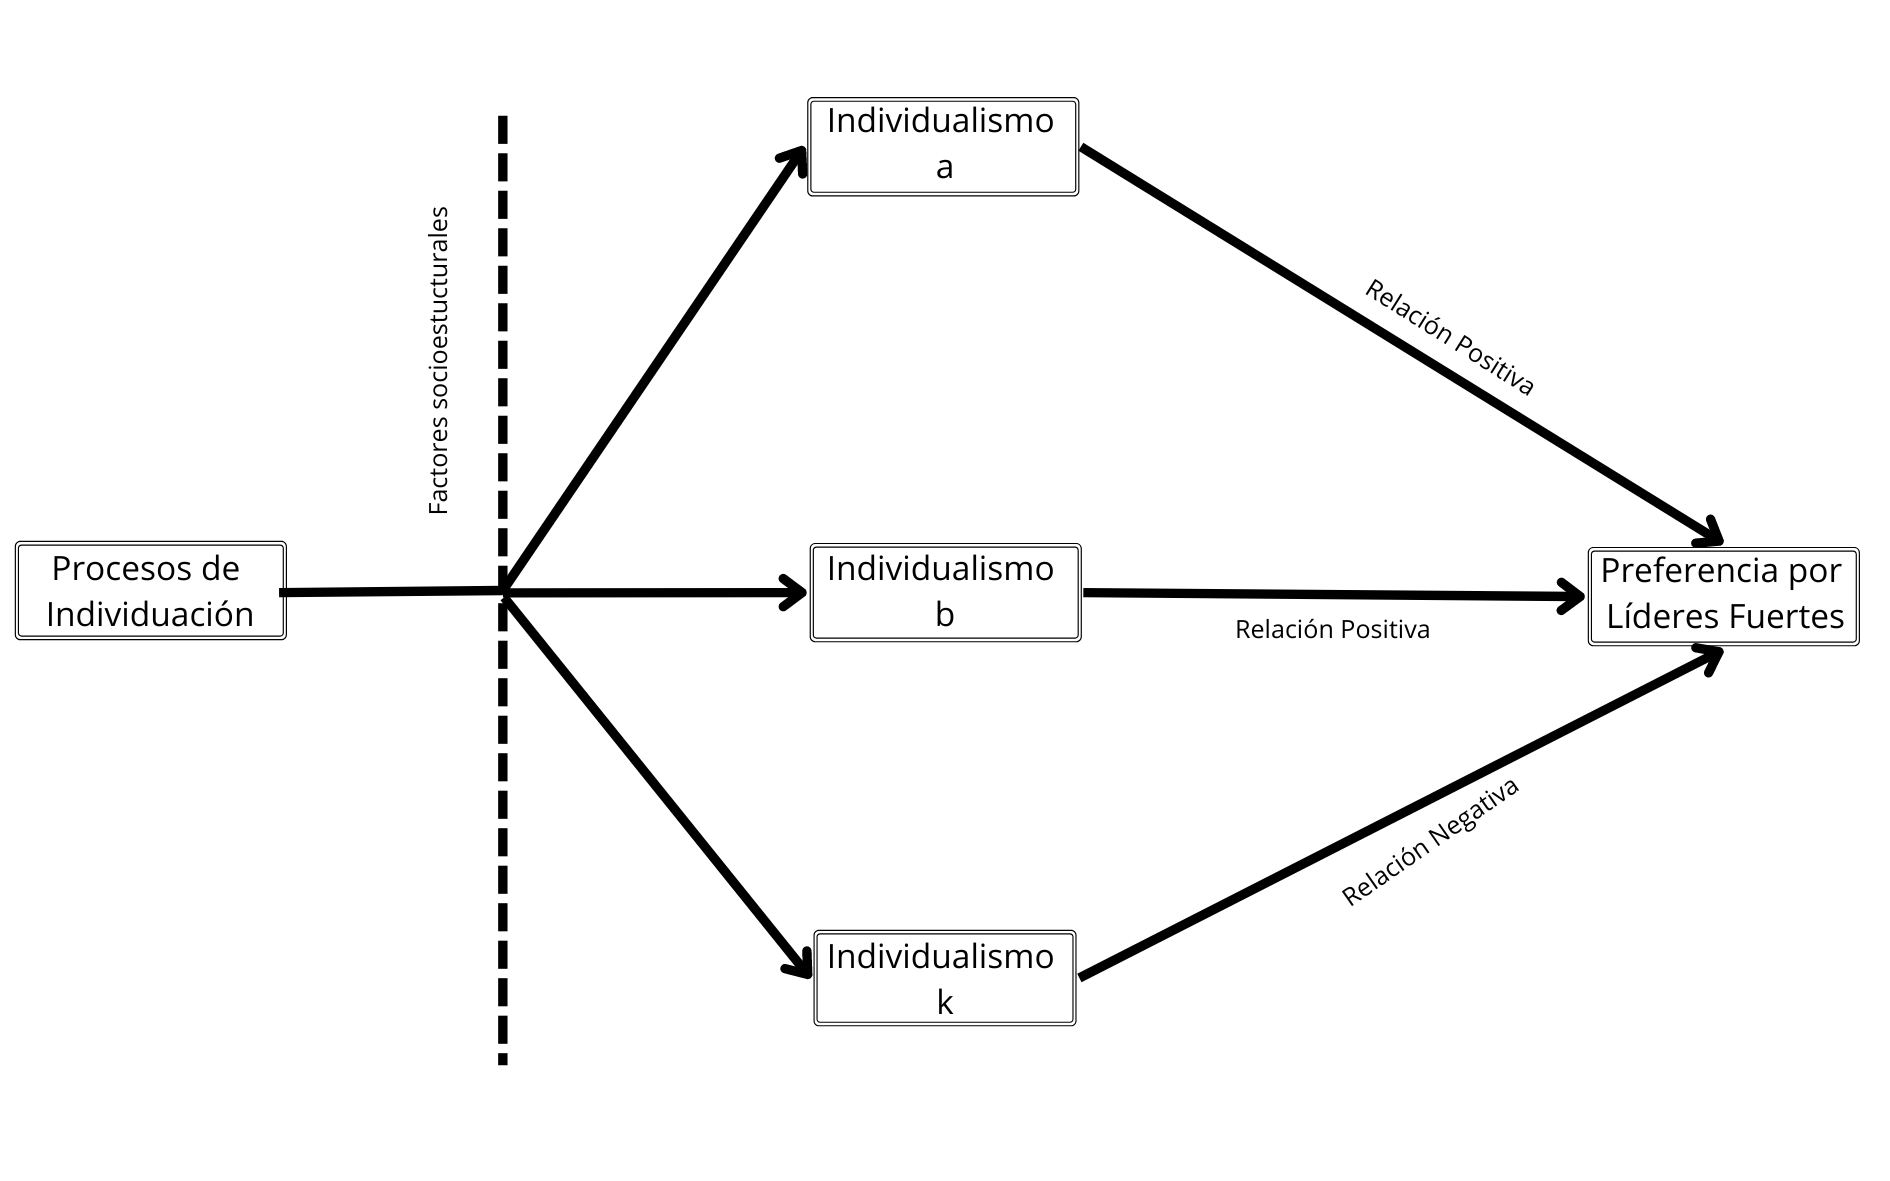
\includegraphics[width=1\linewidth,height=\textheight,keepaspectratio]{images/hipotesis.png}

}

\caption{Modelo Teórico Propuesto}

\end{figure}%

\FloatBarrier

\section*{Estrategia Metodológica}\label{estrategia-metodoluxf3gica}
\addcontentsline{toc}{section}{Estrategia Metodológica}

En esta sección, se presentará la estrategia metodológica que se adoptó
para esta investigación. En primer lugar, se describirán los datos y la
muestra utilizada. Luego, se pasará a describir los indicadores
seleccionados tanto como para la variable independiente como la variable
dependiente, así como las variables de control. Finalmente, se
presentará la estrategia de análisis seguida.

\subsection*{Datos}\label{datos}
\addcontentsline{toc}{subsection}{Datos}

La investigación consistió en un estudio de tipo cuantitativo a partir
de datos secundarios recolectados originalmente para la séptima ola de
la Encuesta Mundial de Valores, que es la más reciente hasta la fecha.
El trabajo de campo en Chile se llevó a cabo en los meses de enero y
febrero de 2018, con una muestra compuesta por 1.000 personas mayores de
18 años, seleccionadas mediante un proceso de muestreo multietápico de
tres niveles. La muestra es representativa a nivel nacional, así como de
áreas urbanas y rurales.

La selección de esta base de datos se fundamenta en que proporciona una
muestra representativa a nivel nacional con indicadores relevantes sobre
valores, creencias y normas sociales, políticas y económicas de la
población. Si bien las preguntas de la Encuesta Mundial de Valores no
fueron pensadas específicamente para el tema de esta investigación, lo
que podría redundar en errores de medición, igualmente resulta posible
construir un modelo que identifique perfiles de individualismo, además
de entregar un buen indicador para medir el apoyo a un líder fuerte. Por
lo tanto, si bien puede limitar el alcance de los resultados obtenidos,
el trabajo con datos secundarios se considera como una solución práctica
ante la limitaciones de esta investigación para producir datos primarios

\FloatBarrier

\subsection*{Variables}\label{variables}
\addcontentsline{toc}{subsection}{Variables}

\subsubsection*{Variable dependiente}\label{variable-dependiente}
\addcontentsline{toc}{subsubsection}{Variable dependiente}

La variable dependiente es el apoyo a un líder fuerte, medido a través
de la valoración sobre qué tan bueno es \emph{tener un líder fuerte que
no se preocupe por el congreso y las elecciones}. La pregunta cuenta con
4 categorías de respuestas (1. Muy bueno; 2. Bueno; 3. Malo; 4. Muy
Malo). Con el fin de incluirla como variable dependiente en un análisis
de regresión logística, como se explicará más adelante, se dicotomizó el
ítem de modo que las dos primeras categorías se entiendan como presencia
de apoyo a un líder fuerte y las dos restantes como ausencia de apoyo.

\subsubsection*{Variable independiente}\label{variable-independiente}
\addcontentsline{toc}{subsubsection}{Variable independiente}

La variable independiente es individualismo, una variable latente y
categórica que fue construida de manera inductiva a partir de un
conjunto de indiciadores operacionalizados en base de las definiciones
teóricas previamente expuestas.

\subparagraph*{Legitimidad de la
individualidad.}\label{legitimidad-de-la-individualidad.}
\addcontentsline{toc}{subparagraph}{Legitimidad de la individualidad.}

Se midió a través de 3 subdimensiones: Legitimidad del individualismo
utilitario, legitimidad del individualismo moral y legitimidad del
individualismo expresivo, siguiendo las distinciones antes introducidas
(\citeproc{ref-cortois2018}{Cortois y Laermans 2018}).

Para la \textbf{legitimidad del individualismo utilitario}, se
seleccionaron indicadores que midan la legitimidad de acciones
estratégicas destinadas a obtener beneficios personales, incluso si
estas acciones van en contra de las normas sociales, tales como la
evasión en el transporte público o la provisión de información falsa
para recibir beneficios sociales. El énfasis aquí se centra en la
legitimidad de poner los fines por sobre los medios. Además, se incluye
un indicador que evalúa la valoración de la competencia, que es una de
las formas principales en que el individualismo utilitario se ha
institucionalizado en las sociedades modernas
(\citeproc{ref-cortois2018}{Cortois y Laermans 2018}).

Para la \textbf{legitimidad del individualismo moral}, se incluyeron
indicadores relacionados con la importancia atribuida a la igualdad de
ingresos, la igualdad de género y los derechos civiles en una
democracia. Con estos, se pretende abordar la importancia que ha
adquirido la igualdad de trato y los derechos humanos en la sociedad
chilena (\citeproc{ref-araujo2012}{Araujo y Martuccelli 2012},
\citeproc{ref-araujo2020a}{2020b}).

Para la \textbf{legitimidad del individualismo expresivo}, se incluyeron
indicadores relacionados con la legitimidad de prácticas
individualizadas en las esferas de la sexualidad y el amor. A pesar de
que el individualismo expresivo se ha extendido a otras áreas de la
sociedad (\citeproc{ref-gauthier2021}{Gauthier 2021}), se considera que
las cristalizaciones más puras del individualismo expresivo se
encuentran en las esferas de la sexualidad y el amor. Bajo la égida del
individualismo expresivo, pues, el matrimonio y los roles sexuales dejan
de estar vinculados a rígidos roles estructurales para pasar a ser el
terreno de la autenticidad y la autoexpresión
(\citeproc{ref-illouz2020}{Illouz 2020}). Por ello, los indicadores
seleccionados abordan temas tales como la homosexualidad, el divorcio y
las relaciones sexuales premaritales.

Estos 9 ítems corresponden a escalas del 1 al 10. Dado que unas de las
técnicas de análisis utilizadas (el análisis de clases latentes, como se
presentará más adelante) requiere que los indicadores del modelo sean
categóricos, y con el objetivo de simplificar el análisis, se ha optado
por dicotomizar estas variables. De tal modo, los valores iguales o
inferiores a 5 se consideraron como una baja justificación de las
acciones mencionadas, mientras que los valores superiores a 5 se
entendieron como una alta justificación \footnote{La única excepción es
  el indicador de competencia, donde los valores se encontraban
  invertidos. Para facilitar el análisis, se recodificó de modo que 2
  indicadora una mayor valoración de la competencia, y 1 una menor.}.

\subparagraph*{Concepciones del
individuo.}\label{concepciones-del-individuo.}
\addcontentsline{toc}{subparagraph}{Concepciones del individuo.}

Se construyó a partir de las 3 subdimensiones definidas por Brewer y
Chen (\citeproc{ref-brewer2007}{2007}): concepción independiente,
concepción relacional, y concepción colectiva.

La \textbf{concepción independiente} se midió a través de un indicador
sobre el grado de control percibido sobre la propia vida, en una escala
del 1 al 10, donde 1 representa ``ningún control'' y 10 ``una gran
cantidad de control''. El ítem ha sido recodificado de modo que los
valores iguales o inferiores a 5 representen un bajo control sobre la
propia vida, mientras que los valores superiores a 5 se entienden como
un alto control.

La \textbf{concepción relacional} se midió a través del grado de acuerdo
con la afirmación ``una de mis metas en la vida ha sido que mis padres
estén orgullosos de mí''. Cabe destacar que la familia es solo una de
las múltiples relaciones cercanas a partir de las que los individuos
pueden definir su identidad. Sin embargo, debido a las limitaciones de
la base de datos y considerando que la familia posiblemente representa
la principal instancia de sociabilidad en la sociedad chilena
(\citeproc{ref-araujo2012}{Araujo y Martuccelli 2012}), se argumenta que
este indicador proporciona una buena aproximación para medir la
interdependencia relacional. Se trata de una escala Likert de 4
categorías, por lo que se optó por mantener la codificación original y
reducir la pérdida de varianza.

La \textbf{concepción colectiva} se midió a través del grado de cercanía
que se siente con el país. Es importante destacar que la identidad
nacional es solo una de las múltiples identidades colectivas que podrían
incluirse en esta subdimensión. Entre éstas, podrían considerarse las
identidades étnicas, religiosas, de clase o territoriales, entre otras.
Sin embargo, la Encuesta Mundial de Valores proporciona datos únicamente
sobre identidades nacionales, regionales y locales. Ahora bien, es
importante mencionar que, en el contexto chileno, la identidad regional
y la identidad nacional están estrechamente relacionadas
(\citeproc{ref-zuniga2010}{Zúñiga y Asún 2010}), por lo que integrar
ambas en el modelo podría resultar redundante. Al igual que el ítem
anterior, se trata de una escala Likert de 4 categorías, por lo se que
mantuvo la codificación original.

\subparagraph*{Valores e Imperativos.}\label{valores-e-imperativos.}
\addcontentsline{toc}{subparagraph}{Valores e Imperativos.}

Posiblemente, esta sea la dimensión de mayor complejidad teórica y que
requiere un cuidado especial en su operacionalización. Afortunadamente,
la Encuesta Mundial de Valores ofrece una solución simple pero adecuada.
El indicador seleccionado consiste en la pregunta: \emph{La mayoría de
las personas consideran que tanto la libertad como la seguridad son
importantes, pero si tuviera que elegir una, ¿cuál consideras que es más
importante?} Este indicador proporciona una forma sencilla de determinar
si la autonomía es el valor principal para los individuos o si se ve
desplazada por el deseo de seguridad.

Los indicadores seleccionados, junto a su operacionalización y su
recodificación, se resumen en la Tabla 1

\begingroup\fontsize{10}{12}\selectfont

\begin{longtable}[t]{>{\centering\arraybackslash}p{3cm}>{\centering\arraybackslash}p{8cm}>{\raggedright\arraybackslash}p{3cm}}
\caption{Resumen indicadores}\\
\toprule
\multicolumn{1}{c}{Dimensión} & \multicolumn{1}{c}{Indicadores} & \multicolumn{1}{c}{Recodificación}\\
\midrule
\addlinespace[0.3em]
\multicolumn{3}{l}{\textbf{Legitimidad de la individualidad}}\\
 &  & 1. Alta acuerdo\\

\nopagebreak
 & \multirow{-2}{8cm}{\centering\arraybackslash La competencia es buena o perjudicial} & 2. Baja acuerdo\\

\nopagebreak
 &  & 1. Alta justificación\\

\nopagebreak
 & \multirow{-2}{8cm}{\centering\arraybackslash Evitar el pago de pasaje en el transporte público} & 2. Baja justificación\\

\nopagebreak
 &  & 1. Alta justificación\\

\nopagebreak
\multirow{-6}{3cm}{\centering\arraybackslash Legitimidad individualismo utilitario} & \multirow{-2}{8cm}{\centering\arraybackslash Exigir beneficios del gobierno a los que no se tiene derecho} & 2. Baja justificación\\

\cmidrule{1-3}\pagebreak[0]
 &  & 1. Alta importancia\\

\nopagebreak
 & \multirow{-2}{8cm}{\centering\arraybackslash El Estado hace que los ingresos de las personas sean iguales} & 2. Baja importancia\\

\nopagebreak
 &  & 1. Alta importancia\\

\nopagebreak
 & \multirow{-2}{8cm}{\centering\arraybackslash Las mujeres tienen los mismos derechos que los hombre} & 2. Baja importancia\\

\nopagebreak
 &  & 1. Alta importancia\\

\nopagebreak
\multirow{-6}{3cm}{\centering\arraybackslash Legitimidad individualismo moral} & \multirow{-2}{8cm}{\centering\arraybackslash Los derechos civiles protegen la libertad de la gente contra la opresión del Estado} & 2. Baja importancia\\

\cmidrule{1-3}\pagebreak[0]
 &  & 1. Alta justificación\\

\nopagebreak
 & \multirow{-2}{8cm}{\centering\arraybackslash La homosexualidad} & 2. Baja justificación\\

\nopagebreak
 &  & 1. Alta justificación\\

\nopagebreak
 & \multirow{-2}{8cm}{\centering\arraybackslash El divorcio} & 2. Baja justificación\\

\nopagebreak
 &  & 1. Alta justificación\\

\nopagebreak
\multirow{-6}{3cm}{\centering\arraybackslash Legitimidad individualismo expresivo} & \multirow{-2}{8cm}{\centering\arraybackslash Tener relaciones sexuales antes del matrimonio} & 2. Baja justificación\\

\cmidrule{1-3}\pagebreak[0]
\addlinespace[0.3em]
\multicolumn{3}{l}{\textbf{Concepciones del Individuo}}\\
 &  & 1. Un gran control\\

\nopagebreak
\multirow{-2}{3cm}{\centering\arraybackslash Concepción Independiente} & \multirow{-2}{8cm}{\centering\arraybackslash ¿Cuánta libertad de elegir y de control siente usted que tiene sobre la forma en que le resulta su vida?} & 2. Nada de control\\

\cmidrule{1-3}\pagebreak[0]
 &  & 1. Muy de acuerdo\\

\nopagebreak
 &  & 2. De acuerdo\\

\nopagebreak
 &  & 3. En desacuerdo\\

\nopagebreak
\multirow{-4}{3cm}{\centering\arraybackslash Concepción Relacional} & \multirow{-4}{8cm}{\centering\arraybackslash Una de mis metas en la vida ha sido que mis padres estén orgullosos de mi} & 4. Muy en desacuerdo\\

\cmidrule{1-3}\pagebreak[0]
 &  & 1. Muy cercano\\

\nopagebreak
 &  & 2. Cercano\\

\nopagebreak
 &  & 3. Poco cercano\\

\nopagebreak
\multirow{-4}{3cm}{\centering\arraybackslash Concepción Colectiva} & \multirow{-4}{8cm}{\centering\arraybackslash Cercanía con Chile} & 4. Nada cercano\\

\cmidrule{1-3}\pagebreak[0]
\addlinespace[0.3em]
\multicolumn{3}{l}{\textbf{Valores e imperativos}}\\
 &  & 1. La Libertad\\

\nopagebreak
\multirow{-2}{3cm}{\centering\arraybackslash Valor principal} & \multirow{-2}{8cm}{\centering\arraybackslash Considera más importante} & 2. La seguridad\\
\bottomrule
\end{longtable}
\endgroup{}

\FloatBarrier

\subsubsection*{Variables de control}\label{variables-de-control}
\addcontentsline{toc}{subsubsection}{Variables de control}

Se incluirán variables de control, principalmente aquellas relacionadas
con características sociodemográficas que se ha observado se relacionan
con el apoyo a la democracia, al populismo o al autoritarismo. De tal
modo, se incluirán en el modelo la autoidentificación política en el
espectro izquierda-derecha, el sexo, la edad, el nivel educacional y la
identificación religiosa y zona de residencia (urbano-rural) y tamaño de
ciudad (\citeproc{ref-navia2019}{Navia y Osorio 2019};
\citeproc{ref-gidron2020}{Gidron y Hall 2020};
\citeproc{ref-eskelinen2020}{Eskelinen y Verkuyten 2020};
\citeproc{ref-schafft2021}{Schafft 2021};
\citeproc{ref-deppisch2022}{Deppisch, Osigus, y Klärner 2022}). Dado que
se ha observado que tanto el estatus socioeconómico subjetivo
(\citeproc{ref-nowakowski2021}{Nowakowski 2021};
\citeproc{ref-gidron2020}{Gidron y Hall 2020}) como objetivo
(\citeproc{ref-xuereb2021}{Xuereb et~al. 2021}), se incluyeron
indicadores para ambos. En el caso del estatus subjetivo, se incluyó la
variable de ingresos subjetivos. Para estatus objetivo, se tomó una
variable sobre grupo ocupacional que puede ser fácilmente recodificada
para aproximarse a los tres grupos principales delineados por el esquema
de clases de Goldthorpe: clase de servicio, clases intermedias y clase
trabajadora (\citeproc{ref-regidor2001}{Regidor 2001}).

Los indicadores seleccionados como variables de control se resumen a
continuación en la tabla 2.

\begingroup\fontsize{12}{14}\selectfont

\begin{ThreePartTable}
\begin{TableNotes}[para]
\item \textit{Nota.} 
\item La variable de posición política correspondía originalmente a una escala del 1 al 10. Entre paréntesis se indican las posiciones que fueron recodificadas para cada categoría
\end{TableNotes}
\begin{longtable}[t]{c>{\raggedright\arraybackslash}p{12cm}}
\caption{Resumen Variables de Control}\\
\toprule
\multicolumn{1}{c}{Variable} & \multicolumn{1}{c}{Categorías}\\
\midrule
 & 1. Hombre\\
\nopagebreak
\multirow{-2}{*}{\centering\arraybackslash Género} & 2. Mujer\\
\cmidrule{1-2}\pagebreak[0]
Edad & Continua\\
\cmidrule{1-2}\pagebreak[0]
 & 1. Ninguna\\
\nopagebreak
 & 2. Izquierda (1 y 2)\\
\nopagebreak
 & 3. Centro Izquierda (3 y 4)\\
\nopagebreak
 & 4. Centro (5)\\
\nopagebreak
 & 5. Centro Derecha (6 a 8)\\
\nopagebreak
\multirow{-6}{*}{\centering\arraybackslash Posición Política} & 6. Derecha (9 y 10)\\
\cmidrule{1-2}\pagebreak[0]
 & 1. Ingresos subjetivos bajos\\
\nopagebreak
\multirow{-2}{*}{\centering\arraybackslash Ingresos Subjetivos} & 10. Ingresos subjetivos altos\\
\cmidrule{1-2}\pagebreak[0]
 & 1. Ninguna\\
\nopagebreak
 & 2. Católica\\
\nopagebreak
 & 3. Evángelica\\
\nopagebreak
\multirow{-4}{*}{\centering\arraybackslash Religión} & 4. Otra\\
\cmidrule{1-2}\pagebreak[0]
 & 1. Santiago\\
\nopagebreak
 & 2. Más de 100.000 hab\\
\nopagebreak
 & 3. Menos de 100.000 hab\\
\nopagebreak
\multirow{-4}{*}{\centering\arraybackslash Tipo de Ciudad} & 4. Rural\\
\cmidrule{1-2}\pagebreak[0]
 & 1. Clase de Servicios (Profesionales y funcionarios administrativos superiores)\\
\nopagebreak
 & 2. Clases Intermedias (Cargos Administrativos medios; pequeños y medianos empresarios)\\
\nopagebreak
\multirow{-3}{*}{\centering\arraybackslash Clase Social} & 3. Clase Trabajadora (Trabajadores manuales o agrícolas, cualificados y no-cualificados)\\
\bottomrule
\insertTableNotes
\end{longtable}
\end{ThreePartTable}
\endgroup{}

\FloatBarrier

\subsection*{Estrategia de análisis}\label{estrategia-de-anuxe1lisis}
\addcontentsline{toc}{subsection}{Estrategia de análisis}

\subsubsection*{Análisis descriptivo}\label{anuxe1lisis-descriptivo}
\addcontentsline{toc}{subsubsection}{Análisis descriptivo}

Para determinar los niveles de apoyo a un líder fuerte en Chile, se
llevó a cabo un análisis descriptivo univariado que examinó la
distribución del ítem seleccionado. Además, y con el fin de poner en
perspectiva los resultados observados por este primer análisis, se
compararon los niveles de apoyo a un líder fuerte en Chile tanto con
otros países de América Latina, así como con olas anteriores en el mismo
país.

\subsubsection*{Análisis de clases
latentes}\label{anuxe1lisis-de-clases-latentes}
\addcontentsline{toc}{subsubsection}{Análisis de clases latentes}

Operacionalmente, se entendió individualismo como una variable latente y
categórica que puede medirse a través de un conjunto de indicadores
observados. Por lo tanto, se empleará un análisis de clases latentes
(LCA) para identificar los perfiles de individualismo en la sociedad
chilena. El LCA es un modelo de variables latentes categóricas, lo que
permite identificar diferencias cualitativas y principios de
organización dentro de la población (\citeproc{ref-collins2010}{Collins
y Lanza 2010}).

El análisis se realizó utilizando el paquete \textbf{poLCA}
(\textbf{po}lytomous Variable \textbf{L}atent \textbf{C}lass
\textbf{A}nalysis) en R. Este paquete permite especificar modelos de
clases latentes de manera eficiente con solo unas pocas líneas de código
y proporciona información valiosa sobre el tamaño de cada clase latente,
las probabilidades posteriores de membresía y criterios para evaluar el
ajuste del modelo, como AIC, BIC y otros
(\citeproc{ref-linzer2011}{Linzer y Lewis 2011}).

La selección del modelo se realizó a partir de la evaluación del ajuste
estadístico de modelos con distintos números de clase mediante el
Criterio de Información Akaike (AIC) y el Criterio de Información
Bayesiano (BIC), además de criterios de interpretatibilidad teórica. AIC
y BIC son dos indicadores de ajuste estadístico relativo que permiten la
comparación de modelos. Un valor más bajo en estos indicadores indica un
mejor ajuste, lo que representa un equilibrio óptimo entre la
complejidad y la parsimonia del modelo
(\citeproc{ref-collins2010}{Collins y Lanza 2010}).

\subsubsection*{Análisis de Varianza y Modelos de
Regresión}\label{anuxe1lisis-de-varianza-y-modelos-de-regresiuxf3n}
\addcontentsline{toc}{subsubsection}{Análisis de Varianza y Modelos de
Regresión}

Para determinar la relación entre los perfiles de individualismo
identificados y el apoyo a un líder fuerte se realizó, en primer lugar,
un ANOVA con el fin de determinar si existen diferencias significativas
en la proporción de apoyo a un líder fuerte para cada grupo de
individualismo.

Una vez comprobadas esas diferencias, se realizó un modelo de regresión
logística para establecer la relación entre los perfiles de
individualismo y el apoyo a un líder fuerte. Para esto, se construyó una
nueva variable categórica de individualismo, asignando a cada caso una
categoría (esto es, un perfil de individualismo) en función de la máxima
probabilidad posterior de membresía estimada por el modelo de clases
latentes.

Suponiendo, pues, que la \(clase_1\) se tomaría como categoría de
referencia, el modelo base de esta investigación quedaría definido por
la siguiente fórmula:

\[log(\frac{\pi_{apoya\_liderfuerte}}
{1-\pi_{apoya\_liderfuerte}}) = \alpha + \beta_1Clase_2 + \beta_2Clase_3 + ... + \beta_kClase_j \]

Esta no es una solución ideal, dado el error asociado a la condición
probabilística de la técnica (\citeproc{ref-collins2010}{Collins y Lanza
2010}), pero al menos es una salida pragmática que permitiría arrojar
luces sobre la asociación entre los dos fenómenos centrales de esta
investigación.

\section*{Discusión}\label{discusiuxf3n}
\addcontentsline{toc}{section}{Discusión}

\textbf{Apoyo a la Líderes Fuertes}

Según datos de la Encuesta Mundial de Valores, el 44\% de la población
chilena consideraría como bueno o muy bueno contar con un líder fuerte
que no le importe el congreso o las elecciones. Si bien esta cifra puede
considerarse como baja en el contexto latinoamericano, donde los niveles
de apoyo a un líder fuerte se encuentran sobre el 50\% en prácticamente
todos los países sondeados en la región, se debe destacar una tendencia
al alza sostenida entre el 2006 y el 2018, creciendo 10 puntos
porcentuales en ese período.

Es importante notar que los datos disponibles son anteriores a fenómenos
sociales de gran importancia que podrían influir en como los ciudadanos
evalúan este tipo de líderes, como el Estallido Social del 2019, la
pandemia por COVID-19, la crisis migratoria y de seguridad, así como la
irrupción de liderazgos autoritarios tanto en el contexto nacional como
latinoamericano. Los datos que pueda entregar la Octava Ola de la
Encuesta Mundial de Valores, que debieran estar disponibles a más tardar
en 2026, van a ser interesantes para constatar si esta tendencia ha
continuado durante el último lustro.

\textbf{Perfiles de Individualismo}

El análisis de clases latentes realizado respalda la hipótesis de que
los procesos de individuación divergen dentro de una misma sociedad. A
partir de los datos examinados, se logró identificar cuatro perfiles
distintos de individualismo en la sociedad chilena: individualismo
autoritario, individualismo conservador, individualismo liberal e
individualismo estratégico. Cada uno de estos perfiles equivale a
variadas representaciones de la posición del individuo en la sociedad, y
son resultado de combinaciones específicas de legitimidad de la acción
individual en diferentes esferas, concepciones variadas del individuo, y
diferentes valores e imperativos estructuralmente producidos. Además, la
presencia de diferencias en edad, orientación política, ubicación
geográfica o afiliación religiosa entre estos perfiles arroja luz sobre
cómo los procesos estructurales interactúan de manera diferenciada con
distintos segmentos de la población.

La tipología elaborada permite establecer un diálogo con la descripción
del individualismo agéntico y el híper-actor relacional propuesto por
Araujo y Martuccelli (\citeproc{ref-araujo2020}{2020a}). Este modelo
presenta dos características fundamentales: en primer lugar, la
confianza depositada en las habilidades personales para afrontar la vida
social, y en segundo lugar, la centralidad de las redes interpersonales.
Estos dos rasgos son observables, al menos de manera parcial,
transversalmente en los cuatro perfiles identificados.

En relación con la confianza en el esfuerzo y las habilidades
personales, esto podría observarse en la alta valoración de la
competencia y los elevados niveles de independencia observados de manera
transversal en todos los perfiles. En términos generales, los datos
sugieren que la mayoría de los chilenos cree poseer las habilidades
necesarias para asumir el control de sus propias vidas.

Lo mismo sucede con los altos niveles de interdepedencia observados a
través de los cuatro perfiles. Cierto es que se mide solo una identidad
relacional (la familiar) y solo una identidad colectiva (la nacional).
Pese a esto, no parece demasiado difícil argumentar la importancia de
estas identidades y que incluirlas en el modelo sirve para un buen
primer acercamiento. También es importante señalar que el carácter
relacional del individualismo chileno parece no entrar en contradicción
con las concepciones independientes, que muestran niveles tan elevados
como los indicadores de interdependencia. Esto es consistente tanto con
las dos características que describen al individualismo agéntico
(\citeproc{ref-araujo2020}{Araujo y Martuccelli 2020a}) como con las
investigaciones sobre el \emph{self-construal} en Chile
(\citeproc{ref-benavides2020}{Benavides y Hur 2020};
\citeproc{ref-kolstad2009}{Kolstad y Horpestad 2009}). Además, ofrece
más respaldo a la idea de que ubicar a Chile en un continuo entre el
individualismo y el colectivismo resulta problemático.

En resumen, a partir de los datos analizados, se puede concluir que el
individualismo agéntico (\citeproc{ref-araujo2020}{Araujo y Martuccelli
2020a}) representa el modelo predominante de individualismo en Chile.
Sin embargo, el aporte de esta investigación radica en que, mediante el
análisis de clases latentes, es posible observar cómo este modelo
diverge dentro de la sociedad chilena. Para algunos, la acción
individual debe estar subordinada al orden normativo, mientras que para
otros es legítimo actuar de manera estratégica incluso si ello
transgrede normas sociales. Mientras que para unos la individualidad
tiene cabida en todas las esferas, para otros su legitimidad no alcanza
para la esfera afectiva. De tal modo, este enfoque permite observar los
matices y las divergencias de los procesos de individualización en
Chile.

\textbf{Apoyo a la democracia delegativa y perfiles de individualismo}

El hecho de que haya sido posible establecer una relación
estadísticamente significativa entre los perfiles de individualismo y el
respaldo a liderazgos fuertes debe ser considerado como una evidencia
alentadora del potencial del modelo teórico de individualismo propuesto.
Dos de los perfiles identificados muestran una asociación negativa con
el apoyo a este tipo de líderes (el conservador y el liberal), mientras
que los otros dos (el estratégico y el autoritario) presentan una
relación positiva. También es importante destacar que aquellos que
muestran mayores niveles de apoyo son justamente quienes presentaban una
menor participación electoral en 2018, en un contexto de voto
voluntario.

Cabe preguntarse si este no es un eje que permita distinguir entre los
perfiles identificados: el individualismo conservador y el liberal
podrían denominarse como \emph{individualismos cívicos}, orientados
hacia lo público. En contraste, el autoritario y el estratégico podrían
considerarse \emph{hiperindividualismos}, que están orientados más bien
hacia lo privado. En los primeros, la individualidad estaría vinculada a
la pertenencia a una comunidad política; en los segundos, lo público
representaría un desafío, un obstáculo que se debe evitar ya sea
mediante la sumisión de la individualidad a un orden normativo (como en
el caso del individualismo autoritario) o mediante la maximización de
las habilidades personales (como es el caso del individualismo
estratégico).

Tomando en consideración las diferencias en participación política entre
los perfiles, cabe reflexionar sobre las consecuencias de estos
hallazgos sobre la democracia chilena, particularmente considerando que
ahora los grupos que muestran un mayor apoyo a los líderes fuertes están
obligados a votar, en un contexto de crisis de seguridad y en que el
denominado ``estilo Bukele'' empieza a ganar adherentes en el país. Si
bien otros estudios (\citeproc{ref-coes2023}{COES 2023}) han notado la
mayor tendencia hacia el autoritarismo y el conservadurismo de los
nuevos votantes, cabe preguntarse si es el único fenómeno aquí presente.
Normalmente, se ha considerado que la sumisión de la autonomía a la
autoridad es un rasgo propio de las personalidades autoritarias
(\citeproc{ref-zakrisson2005}{Zakrisson 2005}). Si bien esto se
observaría en el individualismo autoritario, no es el caso el
individualismo estratégico ¿Porque un grupo de la población que valora y
legitima la acción individual en todas las esferas estaría predispuesto
a liderazgos dominantes?

Una respuesta se puede encontrar en, como se menciona en la Encuesta
Nacional de la Autoridad (\citeproc{ref-araujo2022}{Araujo et~al.
2022}), la autoridad política estaría sostenida en la eficacia de los
liderazgos para cumplir sus tareas. Esto en un contexto que Juan Pablo
Luna (\citeproc{ref-luna2016}{2016}) ha denominado como ``Democracia
Desarraigada'', donde existe una fuerte desconexión entre ciudadanos y
élite política. De tal modo, sería posible hipotetizar que el deseo de
los chilenos -- particularmente de los \emph{hiperindividualistas} --
por liderazgos fuertes no es puro autoritarismo, sino la demanda por un
tipo de autoridad que se podría denominar como \emph{delegativa}
(\citeproc{ref-odonnell1994}{O'Donnell 1994}). En una democracia
delegativa, los ciudadanos podrían ejercer el voto periódicamente para
luego retirarse de la esfera pública hasta la próxima elección
(\citeproc{ref-peruzzotti2008}{Peruzzotti 2008}). Pero esta apatía está
lejos de ser un cheque en blanco: al líder electo se le exigen
resultados, incluso si ello implica transgredir la autonomía de otras
instituciones del Estado. Los hiperindividualistas, así, no estarían --
necesariamente -- en contra de la democracia, pero sí tendrían una
visión más pragmática de esta.

En resumen, esta investigación sugiere que la relación entre el
individualismo y el apoyo a líderes fuertes es significativa, pero
divergente entre distintos grupos. En otras palabras, distintas formas
de individualismos, resultado de divergencias en los procesos de
individuación, preferirían formas distintas de ejercer la autoridad.
Mientras que los individualismos cívicos parecen valorar una visión más
representativa de la democracia, los hiperindividualismos favorecen un
enfoque más pragmático y apático hacia la esfera pública. Esto ilustra
un panorama general en el que las manifestaciones del individualismo, y
su relación con otros fenómenos, aparecen como más complejas de lo que
otros estudios han propuesto.

\section*{Conclusión}\label{conclusiuxf3n}
\addcontentsline{toc}{section}{Conclusión}

Es importante reflexionar sobre las oportunidades que brinda el análisis
de clases latentes en la investigación sobre los procesos de
individuación en Chile. Dada la dificultad para traducir su marco
teórico a una propuesta metodológica mediante las técnicas cuantitativas
más comunes, la sociología del individuo se ha desarrollado
principalmente desde una perspectiva cualitativa, resultando en
descripciones profundas y estimulantes sobre el individuo en la sociedad
chilena. Pese a ello, el enfoque metodológico adoptado en esta
investigación permitió identificar algunos de los rasgos del
individualismo agéntico descritos por Araujo y Martuccelli
(\citeproc{ref-araujo2014}{2014}), al tiempo que ofrece una visión más
matizada de cómo los procesos de individuación divergen en la sociedad
chilena, diferenciándose entre grupos sociales y teniendo consecuencias
en las actitudes políticas de los individuos.

Por supuesto, enfoques cualitativos y cuantitativos no deben ser vistos
como competitivos, sino como complementarios en el desarrollo de una
sociología del individuo. Las propias conclusiones aquí delineadas, y
las hipótesis que de ellas se desprenden, se verían fuertemente
enriquecidas si se incluyeran datos cualitativos que permitieran obtener
una compresión más profunda de las distintas variantes de individualismo
y su relación divergente con la esfera pública.

Ahora bien, es necesario reconocer las limitaciones que enfrentó esta
investigación, principalmente derivadas de los indicadores
seleccionados. Aunque los resultados obtenidos parecen prometedores, es
crucial continuar avanzando en la construcción y validación de
indicadores que permitan traducir el modelo teórico aquí propuesto en un
modelo de medición capaz de abordar el fenómeno del individualismo en
Chile. En particular, las operacionalizaciones del individualismo
utilitario, del individualismo moral, de la interdependencia relacional
y de la interdependencia colectiva merecen, sin duda, un mayor trabajo
metodológico y conceptual que permitan construir y validar indicadores
en esas dimensiones.

Por otro lado, la recodificación de variables continuas como dicotómicas
es una solución correcta, pero que no deja de ser problemática, ya que
resulta en la pérdida de parte de la varianza de los ítems
(\citeproc{ref-fernandes2019}{Fernandes et~al. 2019}). Futuras
investigaciones deberían considerar elaborar indicadores directamente
como variables categóricas que no necesiten recodificación para ser
incluidas en el modelo de clases latentes. De esta manera, se obtendría
claridad en los resultados sin sacrificar información ni poder
estadístico.

Otras limitaciones provienen más bien de la muestra. Si 5 años ya se
encuentra en el límite de lo que se puede considerar como datos
relevantes para la actualidad, a esto se debe sumar que este último
lustro ha sido uno particularmente tumultuoso: el Estallido Social, la
Pandemia, el proceso constituyente, la crisis migratoria y la crisis de
seguridad han sido algunos de los eventos de gran magnitud que han
marcado la agenda durante los últimos años. ¿Están hoy los chilenos más
dispuestos que hace 5 años a sacrificar su libertad y su individualidad
en distintas esferas para obtener garantías de orden y seguridad? Entre
las ollas comunes y los retiros de fondos previsionales, entre las
protestas masivas y las cuarentenas, ¿cambiaron las concepciones --
independientes, relacionales y colectivas -- con las que los individuos
construyen sus identidades? ¿Qué efectos puede tener la instauración del
voto obligatorio en el eje individualismo cívico-hiperindividualismo, o
en las percepciones de los ciudadanos sobre las formas en que se ejerce
la autoridad? Todas estas son preguntas relevantes que quedarán abiertas
y deberán ser abordadas en el futuro.

A su vez, dado que Chile ha participado en 6 olas de la Encuesta Mundial
de Valores desde 1990, se debería considerar correr los modelos aquí
propuestos utilizando datos de ediciones anteriores (así como estar
atentos a la próxima versión a realizarse entre 2023 y 2026). Esto
permitiría evaluar si los resultados obtenidos en este estudio guardan
consistencia con el pasado, así como observar la evolución de estos
indicadores a lo largo del tiempo.

Pese a estas limitaciones, el trabajo contenido en este documento logra
obtener resultados relevantes. Se encontró evidencia de que distintas
formas de individualismo pueden generar actitudes políticas diferentes
respecto a los tipos de liderazgos esperados por la ciudadanía. Es
importante considerar que estas inclinaciones no surgen en un vacío,
sino que son el resultado de la interacción de factores institucionales
y estructurales con la agencia de los individuos. De esta manera, se
espera que la lectura de esta investigación provoque la reflexión en
torno a los tipos de individuos que nuestras instituciones, a través de
sus programas e incentivos, contribuyen a producir, así como en las
consecuencias de estos procesos para la democracia chilena y la vida
social en general.

\textbf{Palabras finales}

Este documento es resultado de la investigación desarrollado en el marco
de mi tesis para obtener el grado de Magíster en Métodos para la
Investigación Social en la Universidad Diego Portales. Quisiera
agradecer especialmente a la profesora Macarena Orchard por su guía en
este proceso. También agradezco a los comentarios de los profesores
Carlos Meléndez y Cristóbal Moya por sus comentarios que ayudaron a
mejorar este artículo.

\phantomsection\label{refs}
\begin{CSLReferences}{1}{0}
\bibitem[\citeproctext]{ref-araujo2021}
Araujo, Kathya. 2021. \emph{{\textquestiondown}{C{ó}mo Estudiar} La
Autoridad?} USACH.

\bibitem[\citeproctext]{ref-araujo2022a}
---------. 2022. {«Introducci{ó}n. {Las} Figuras de Autoridad y El
Vendaval»}. En \emph{Figuras de Autoridad. {Transformaciones}
Hist{ó}ricas y Ejercicios Contempor{á}neos}, 11-29. LOM.

\bibitem[\citeproctext]{ref-araujo2012}
Araujo, Kathya, y Danilo Martuccelli. 2012. \emph{Desaf{í}os {Comunes}.
{Retrato} de La Sociedad Chilena y Sus Individuos}. LOM.

\bibitem[\citeproctext]{ref-araujo2014}
---------. 2014. {«Beyond Institutional Individualism: {Agentic}
Individualism and the Individuation Process in {Chilean} Society»}.
\emph{Current Sociology} 62 (1): 24-40.
\url{https://doi.org/10.1177/0011392113512496}.

\bibitem[\citeproctext]{ref-araujo2020}
---------. 2020a. {«Leer Los Movimientos Sociales Desde El
Individualismo: {Reflexiones} a Partir de {Latinoam{é}rica}»}.
\emph{Educa{ç}{ã}o \& Sociedade} 41: e228265.
\url{https://doi.org/10.1590/es.228265}.

\bibitem[\citeproctext]{ref-araujo2020a}
---------. 2020b. {«Problematizaciones Del Individualismo En {Am{é}rica
Latina}»}. \emph{Perfiles Latinoamericanos} 28 (55).
\url{https://doi.org/10.18504/pl2855-001-2020}.

\bibitem[\citeproctext]{ref-araujo2022}
Araujo, Kathya, Macarena Orchard, Alejandra Rasse, y Antonio Stecher.
2022. {«Primer {Informe} de {Resultados Encuesta Nacional} de {Autoridad
NUMAAP} 2021»}. Santiago de Chile: NUMAAP.

\bibitem[\citeproctext]{ref-arikan2019}
Arikan, Gizem, y Eser Sekercioglu. 2019. {«Authoritarian
{Predispositions} and {Attitudes Towards Redistribution}»}.
\emph{Political Psychology} 40 (5): 1099-1118.
\url{https://doi.org/10.1111/pops.12580}.

\bibitem[\citeproctext]{ref-armendarizmiranda2021}
Armendariz Miranda, Paula, y Matthew Cawvey. 2021. {«Introverted and
{Closed-Minded}: {The Psychological Roots} of {Support} for {Autocracy}
in {Latin America}»}. \emph{Journal of Politics in Latin America} 13
(1): 40-66. \url{https://doi.org/10.1177/1866802X21991261}.

\bibitem[\citeproctext]{ref-baro2022}
Baro, Elena. 2022. {«Personal {Values Priorities} and {Support} for
{Populism} in {Europe}---{An Analysis} of {Personal Motivations
Underpinning Support} for {Populist Parties} in {Europe}»}.
\emph{Political Psychology} 43 (6): 1191-1215.
\url{https://doi.org/10.1111/pops.12812}.

\bibitem[\citeproctext]{ref-benavides2020}
Benavides, Paloma, y Taekyun Hur. 2020. {«Self-{Construal Differences}
in {Chile} and {South Korea}: {A Brief Report}»}. \emph{Psychological
Reports} 123 (6): 2410-17.
\url{https://doi.org/10.1177/0033294119868786}.

\bibitem[\citeproctext]{ref-brewer2007}
Brewer, Marilynn B., y Ya-Ru Chen. 2007. {«Where ({Who}) {Are
Collectives} in {Collectivism}? {Toward Conceptual Clarification} of
{Individualism} and {Collectivism}.»} \emph{Psychological Review} 114
(1): 133-51. \url{https://doi.org/10.1037/0033-295X.114.1.133}.

\bibitem[\citeproctext]{ref-brunkert2023}
Brunkert, Lennart, y Christian Von Soest. 2023. {«Praising the Leader:
Personalist Legitimation Strategies and the Deterioration of Executive
Constraints»}. \emph{Democratization} 30 (3): 419-39.
\url{https://doi.org/10.1080/13510347.2022.2150760}.

\bibitem[\citeproctext]{ref-cadem2023}
CADEM. 2023. {«Encuesta {Plaza P{ú}blica}. {Cuarta Semana} de
{Febrero}»}. CADEM.

\bibitem[\citeproctext]{ref-carlin2011}
Carlin, Ryan E. 2011. {«Distrusting {Democrats} and {Political
Participation} in {New Democracies}: {Lessons} from {Chile}»}.
\emph{Political Research Quarterly} 64 (3): 668-87.
\url{https://doi.org/10.1177/1065912910370692}.

\bibitem[\citeproctext]{ref-carlin2018}
---------. 2018. {«Sorting {Out Support} for {Democracy}: {A Q-Method
Study}: {Q-Sorting Democratic Support}»}. \emph{Political Psychology} 39
(2): 399-422. \url{https://doi.org/10.1111/pops.12409}.

\bibitem[\citeproctext]{ref-cep}
CEP. 2023. {«Encuesta {CEP N}{\(^\circ\)}88, {Noviembre-Diciembre}
2022»}. Centro de Estudios P{ú}blicos.

\bibitem[\citeproctext]{ref-cerc-mori}
CERC-MORI. 2023. {«Chile a La Sombra de {Pinochet}. {La} Opini{ó}n
P{ú}blica Sobre La "{Era} de {Pinochet}" 1973-2022»}. MORI Market
Opinion Research International.

\bibitem[\citeproctext]{ref-coes2023}
COES. 2023. {«Radiograf{í}a Del {Cambio Social} En {Chile} 2016-2022.
{Estudio Longitudinal Social} de {Chile}. {Presentaci{ó}n} de
{Resultados COES}.»} Santiago de Chile: Centro de Estudios de Conflicto
y Cohesi{ó}n Social.

\bibitem[\citeproctext]{ref-collins2010}
Collins, Linda, y Stephanie Lanza. 2010. \emph{Latent Class and Latent
Tansition Analysis.} Wiley.

\bibitem[\citeproctext]{ref-cortois2018}
Cortois, Liza, y Rudi Laermans. 2018. {«Rethinking Individualization:
{The} Basic Script and the Three Variants of Institutionalized
Individualism»}. \emph{European Journal of Social Theory} 21 (1): 60-78.
\url{https://doi.org/10.1177/1368431017698474}.

\bibitem[\citeproctext]{ref-crimston2022}
Crimston, Charlie R., Hema Preya Selvanathan, y Jolanda Jetten. 2022.
{«Moral {Polarization Predicts Support} for {Authoritarian} and
{Progressive Strong Leaders} via the {Perceived Breakdown} of
{Society}»}. \emph{Political Psychology} 43 (4): 671-91.
\url{https://doi.org/10.1111/pops.12787}.

\bibitem[\citeproctext]{ref-cross2011}
Cross, Susan E., Erin E. Hardin, y Berna Gercek-Swing. 2011. {«The
{\emph{What}}{\emph{,} }{\emph{How}}{\emph{,} }{\emph{Why}}{\emph{, and}
}{\emph{Where}} of {Self-Construal}»}. \emph{Personality and Social
Psychology Review} 15 (2): 142-79.
\url{https://doi.org/10.1177/1088868310373752}.

\bibitem[\citeproctext]{ref-deppisch2022}
Deppisch, Larissa, Torsten Osigus, y Andreas Klärner. 2022. {«How
{Rural} Is {Rural Populism}? {On} the {Spatial Understanding} of
{Rurality} for {Analyses} of {Right}-Wing {Populist Election Success} in
{Germany}*»}. \emph{Rural Sociology} 87 (S1): 692-714.
\url{https://doi.org/10.1111/ruso.12397}.

\bibitem[\citeproctext]{ref-diaz2023}
Díaz, Camila, Cristóbal Rovira Kaltwasser, y Lisa Zanotti. 2023. {«The
Arrival of the Populist Radical Right in {Chile}: {Jos{é} Antonio Kast}
and the {``{Partido Republicano}''}»}. \emph{Journal of Language and
Politics} 22 (3): 342-59. \url{https://doi.org/10.1075/jlp.22131.dia}.

\bibitem[\citeproctext]{ref-donovan2019}
Donovan, Todd. 2019. {«Authoritarian Attitudes and Support for Radical
Right Populists»}. \emph{Journal of Elections, Public Opinion and
Parties} 29 (4): 448-64.
\url{https://doi.org/10.1080/17457289.2019.1666270}.

\bibitem[\citeproctext]{ref-donovan2021}
---------. 2021. {«Right Populist Parties and Support for Strong
Leaders»}. \emph{Party Politics} 27 (5): 858-69.
\url{https://doi.org/10.1177/1354068820920853}.

\bibitem[\citeproctext]{ref-eskelinen2020}
Eskelinen, Viivi, y Maykel Verkuyten. 2020. {«Support for Democracy and
Liberal Sexual Mores Among {Muslims} in {Western Europe}»}.
\emph{Journal of Ethnic and Migration Studies} 46 (11): 2346-66.
\url{https://doi.org/10.1080/1369183X.2018.1521715}.

\bibitem[\citeproctext]{ref-fernandes2019}
Fernandes, Antônio, Caio Malaquias, Dalson Figueiredo, Enivaldo Da
Rocha, y Rodrigo Lins. 2019. {«Why {Quantitative Variables Should Not Be
Recoded} as {Categorical}»}. \emph{Journal of Applied Mathematics and
Physics} 07 (07): 1519-30.
\url{https://doi.org/10.4236/jamp.2019.77103}.

\bibitem[\citeproctext]{ref-gauthier2021}
Gauthier, François. 2021. {«{Authenticity, Consumer Culture and
Charismatic Authority \textsuperscript{1}}»}. \emph{Studies in
Religion/Sciences Religieuses} 50 (1): 27-49.
\url{https://doi.org/10.1177/0008429820920885}.

\bibitem[\citeproctext]{ref-gelfand1996}
Gelfand, Michele J., Harry C. Triandis, y Darius K-S. Chan. 1996.
{«Individualism Versus Collectivism or Versus Authoritarianism?»}
\emph{European Journal of Social Psychology} 26 (3): 397-410.
\url{https://doi.org/10.1002/(SICI)1099-0992(199605)26:3\%3C397::AID-EJSP763\%3E3.0.CO;2-J}.

\bibitem[\citeproctext]{ref-gidron2020}
Gidron, Noam, y Peter A. Hall. 2020. {«Populism as a {Problem} of
{Social Integration}»}. \emph{Comparative Political Studies} 53 (7):
1027-59. \url{https://doi.org/10.1177/0010414019879947}.

\bibitem[\citeproctext]{ref-harms2018}
Harms, P. D., Dustin Wood, Karen Landay, Paul B. Lester, y Gretchen
Vogelgesang Lester. 2018. {«Autocratic Leaders and Authoritarian
Followers Revisited: {A} Review and Agenda for the Future»}. \emph{The
Leadership Quarterly} 29 (1): 105-22.
\url{https://doi.org/10.1016/j.leaqua.2017.12.007}.

\bibitem[\citeproctext]{ref-hogg2021}
Hogg, Michael A. 2021. {«Uncertain {Self} in a {Changing World}: {A
Foundation} for {Radicalisation}, {Populism}, and {Autocratic
Leadership}»}. \emph{European Review of Social Psychology} 32 (2):
235-68. \url{https://doi.org/10.1080/10463283.2020.1827628}.

\bibitem[\citeproctext]{ref-hogg2013}
Hogg, Michael A., y Janice Adelman. 2013. {«Uncertainty--{Identity
Theory}: {Extreme Groups}, {Radical Behavior}, and {Authoritarian
Leadership}»}. \emph{Journal of Social Issues} 69 (3): 436-54.
\url{https://doi.org/10.1111/josi.12023}.

\bibitem[\citeproctext]{ref-illouz2020}
Illouz, Eva. 2020. \emph{El Fin Del Amor. {Una} Sociolog{í}a de Las
Relaciones Negativas.} Katz.

\bibitem[\citeproctext]{ref-kang2018}
Kang, Youngho, y Dongwon Lee. 2018. {«Delegative Democratic Attitudes:
{Theory} and Evidence from the {Asian} Barometer Survey»}.
\emph{International Political Science Review} 39 (4): 455-72.
\url{https://doi.org/10.1177/0192512117702755}.

\bibitem[\citeproctext]{ref-kemmelmeier2003}
Kemmelmeier, Markus, Eugene Burnstein, Krum Krumov, Petia Genkova, Chie
Kanagawa, Matthew S. Hirshberg, Hans-Peter Erb, Grazyna Wieczorkowska, y
Kimberly A. Noels. 2003. {«Individualism, {Collectivism}, and
{Authoritarianism} in {Seven Societies}»}. \emph{Journal of
Cross-Cultural Psychology} 34 (3): 304-22.
\url{https://doi.org/10.1177/0022022103034003005}.

\bibitem[\citeproctext]{ref-kendall-taylor2017}
Kendall-Taylor, Andrea, Erica Frantz, y Joseph Wright. 2017. {«The
{Global Rise} of {Personalized Politics}: {It}'s {Not Just Dictators
Anymore}»}. \emph{The Washington Quarterly} 40 (1): 7-19.
\url{https://doi.org/10.1080/0163660X.2017.1302735}.

\bibitem[\citeproctext]{ref-kolstad2009}
Kolstad, Arnulf, y Silje Horpestad. 2009. {«Self-{Construal} in {Chile}
and {Norway}: {Implications} for {Cultural Differences} in
{Individualism} and {Collectivism}»}. \emph{Journal of Cross-Cultural
Psychology} 40 (2): 275-81.
\url{https://doi.org/10.1177/0022022108328917}.

\bibitem[\citeproctext]{ref-kyriacou2016}
Kyriacou, Andreas P. 2016. {«Individualism--Collectivism, Governance and
Economic Development»}. \emph{European Journal of Political Economy} 42
(marzo): 91-104. \url{https://doi.org/10.1016/j.ejpoleco.2015.11.005}.

\bibitem[\citeproctext]{ref-lima2021}
Lima, Marcus E. O., Dalila X. De França, Jolanda Jetten, Cícero R.
Pereira, Michael J. A. Wohl, Inga Jasinskaja-Lahti, Ying-yi Hong, et~al.
2021. {«Materialist and Post-Materialist Concerns and the Wish for a
Strong Leader in 27 Countries»}. \emph{Journal of Social and Political
Psychology} 9 (1): 207-20. \url{https://doi.org/10.5964/jspp.6213}.

\bibitem[\citeproctext]{ref-lindstaedt2021}
Lindstaedt, Natasha. 2021. {«The {Current Landscape}»}. En
\emph{Democratic {Decay} and {Authoritarian Resurgence}}, 17-61.
Bristol, Reino Unido: Bristol University Press.

\bibitem[\citeproctext]{ref-linzer2011}
Linzer, Drew A., y Jeffrey B. Lewis. 2011. {«{poLCA}: {An R Package} for
{Polytomous Variable Latent Class Analysis}»}. \emph{Journal of
Statistical Software} 42 (junio): 1-29.
\url{https://doi.org/10.18637/jss.v042.i10}.

\bibitem[\citeproctext]{ref-luna2016}
Luna, Juan Pablo. 2016. {«Chile's {Crisis} of {Representation}»}.
\emph{Journal of Democracy} 27 (3): 129-38.
\url{https://doi.org/10.1353/jod.2016.0046}.

\bibitem[\citeproctext]{ref-marchlewska2019}
Marchlewska, Marta, Kevin A. Castellanos, Karol Lewczuk, Mirosław Kofta,
y Aleksandra Cichocka. 2019. {«My Way or the Highway: {High} Narcissism
and Low Self-Esteem Predict Decreased Support for Democracy»}.
\emph{British Journal of Social Psychology} 58 (3): 591-608.
\url{https://doi.org/10.1111/bjso.12290}.

\bibitem[\citeproctext]{ref-marchlewska2022}
Marchlewska, Marta, Aleksandra Cichocka, Aleksandra Furman, y Aleksandra
Cislak. 2022. {«Who Respects the Will of the People? {Support} for
Democracy Is Linked to High Secure National Identity but Low National
Narcissism»}. \emph{British Journal of Social Psychology} 61 (2):
599-621. \url{https://doi.org/10.1111/bjso.12499}.

\bibitem[\citeproctext]{ref-martuccelli2010}
Martuccelli, Danilo. 2010. \emph{{{\textquestiondown}Existen individuos
en el sur?}} Santiago de Chile: LOM.

\bibitem[\citeproctext]{ref-martuccelli2018}
---------. 2018. {«Variantes Del Individualismo»}. \emph{Estudios
Sociol{ó}gicos de El Colegio de M{é}xico} 37 (109): 7-37.
\url{https://doi.org/10.24201/es.2019v37n109.1732}.

\bibitem[\citeproctext]{ref-moemeka1998}
Moemeka, Andrew A. 1998. {«Communalism as a {Fundamental Dimension} of
{Culture}»}. \emph{Journal of Communication} 48 (4): 118-41.
\url{https://doi.org/10.1111/j.1460-2466.1998.tb02773.x}.

\bibitem[\citeproctext]{ref-navia2019}
Navia, Patricio, y Rodrigo Osorio. 2019. {«Attitudes Toward Democracy
and Authoritarianism Before, During and After Military Rule. {The} Case
of {Chile}, 1972--2013»}. \emph{Contemporary Politics} 25 (2): 190-212.
\url{https://doi.org/10.1080/13569775.2018.1504426}.

\bibitem[\citeproctext]{ref-nowakowski2021}
Nowakowski, Adam. 2021. {«Do Unhappy Citizens Vote for Populism?»}
\emph{European Journal of Political Economy} 68 (junio): 101985.
\url{https://doi.org/10.1016/j.ejpoleco.2020.101985}.

\bibitem[\citeproctext]{ref-odonnell1994}
O'Donnell, Guillermo A. 1994. {«Delegative {Democracy}»}. \emph{Journal
of Democracy} 5 (1): 55-69. \url{https://doi.org/10.1353/jod.1994.0010}.

\bibitem[\citeproctext]{ref-oyserman2002}
Oyserman, Daphna, Heather M. Coon, y Markus Kemmelmeier. 2002.
{«Rethinking Individualism and Collectivism: {Evaluation} of Theoretical
Assumptions and Meta-Analyses.»} \emph{Psychological Bulletin} 128 (1):
3-72. \url{https://doi.org/10.1037/0033-2909.128.1.3}.

\bibitem[\citeproctext]{ref-peruzzotti2008}
Peruzzotti, Enrique. 2008. {«Populismo y Representaci{ó}n
Democr{á}tica»}. En \emph{El Retorno Del Pueblo. {Populismo} y Nuevas
Democracias En {Am{é}rica Latina}.}, editado por Carlos de la Torre y
Enrique Peruzzotti, 97-124. FLACSO Ecuador.

\bibitem[\citeproctext]{ref-regidor2001}
Regidor, Enrique. 2001. {«{La clasificaci{ó}n de clase social de
Goldthorpe: marco de referencia para la propuesta de medici{ó}n de la
clase social del grupo de trabajo de la Sociedad Espa{ñ}ola de
Epidemiolog{í}a}»}. \emph{Revista Espa{ñ}ola de Salud P{ú}blica} 75 (1).
\url{https://doi.org/10.1590/S1135-57272001000100003}.

\bibitem[\citeproctext]{ref-rico2020}
Rico, Guillem, Marc Guinjoan, y Eva Anduiza. 2020. {«Empowered and
Enraged: {Political} Efficacy, Anger and Support for Populism in
{Europe}»}. \emph{European Journal of Political Research} 59 (4):
797-816. \url{https://doi.org/10.1111/1475-6765.12374}.

\bibitem[\citeproctext]{ref-robles2001}
Robles, Fernando. 2001. \emph{El Desaliento Inesperado de La Modernidad:
Molestias, Irritaciones y Frutos Amargos de La Sociedad Del Riesgo}.
Sociedad de Hoy.

\bibitem[\citeproctext]{ref-rojas2008}
Rojas-Méndez, José I., Vilma Coutiño-Hill, Rabi S. Bhagat, y Karen South
Moustafa. 2008. {«{Evaluaci{ó}n del individualismo y colectivismo
horizontal y vertical en la sociedad Chilena.}»} \emph{Multidisciplinary
Business Review} 1 (1): 36-48.

\bibitem[\citeproctext]{ref-schafft2021}
Schafft, Kai A. 2021. {«Rurality and {Crises} of {Democracy}: {What Can
Rural Sociology Offer} the {Present Moment}?*»}. \emph{Rural Sociology}
86 (3): 393-418. \url{https://doi.org/10.1111/ruso.12408}.

\bibitem[\citeproctext]{ref-selvanathan2022}
Selvanathan, Hema Preya, Charlie R. Crimston, y Jolanda Jetten. 2022.
{«How Being Rooted in the Past Can Shape the Future: {The} Role of
Social Identity Continuity in the Wish for a Strong Leader»}. \emph{The
Leadership Quarterly} 33 (4): 101608.
\url{https://doi.org/10.1016/j.leaqua.2022.101608}.

\bibitem[\citeproctext]{ref-silvapalacios2015}
Silva Palacios, Vicente. 2015. {«Narrativas de {Individualizaci{ó}n} En
{Chile}»}. Tesis de \{\{Pregrado\}\}, Universidad de Chile.

\bibitem[\citeproctext]{ref-sprong2019}
Sprong, Stefanie, Jolanda Jetten, Zhechen Wang, Kim Peters, Frank Mols,
Maykel Verkuyten, Brock Bastian, et~al. 2019. {«{``{Our Country Needs} a
{Strong Leader Right Now}''}: {Economic Inequality Enhances} the {Wish}
for a {Strong Leader}»}. \emph{Psychological Science} 30 (11): 1625-37.
\url{https://doi.org/10.1177/0956797619875472}.

\bibitem[\citeproctext]{ref-strunk1999}
Strunk, Daniel R, y Edward C Chang. 1999. {«Distinguishing Between
Fundamental Dimensions of Individualism--Collectivism:»}
\emph{Personality and Individual Differences} 27 (4): 665-71.
\url{https://doi.org/10.1016/S0191-8869(98)00258-X}.

\bibitem[\citeproctext]{ref-voronov2002}
Voronov, Maxim, y Jefferson A. Singer. 2002. {«The {Myth} of
{Individualism-Collectivism}: {A Critical Review}»}. \emph{The Journal
of Social Psychology} 142 (4): 461-80.
\url{https://doi.org/10.1080/00224540209603912}.

\bibitem[\citeproctext]{ref-wang2010}
Wang, Georgette, y Zhong-Bo Liu. 2010. {«What Collective? {Collectivism}
and Relationalism from a {Chinese} Perspective»}. \emph{Chinese Journal
of Communication} 3 (1): 42-63.
\url{https://doi.org/10.1080/17544750903528799}.

\bibitem[\citeproctext]{ref-wu2019}
Wu, Wen-Chin, y Yu-Tzung Chang. 2019. {«Income Inequality, Distributive
Unfairness, and Support for Democracy: Evidence from {East Asia} and
{Latin America}»}. \emph{Democratization} 26 (8): 1475-92.
\url{https://doi.org/10.1080/13510347.2019.1656198}.

\bibitem[\citeproctext]{ref-xuereb2021}
Xuereb, Silas, Michael J. A. Wohl, Anna Stefaniak, y Frank J. Elgar.
2021. {«Social and Economic Determinants of Support for a Strong
Non-Democratic Leader in Democracies Differ from Non-Democracies»}.
\emph{Journal of Social and Political Psychology} 9 (2): 334-52.
\url{https://doi.org/10.5964/jspp.7235}.

\bibitem[\citeproctext]{ref-yoon2010}
Yoon, Kwang-Il. 2010. {«Political {Culture} of {Individualism} and
{Collectivism}»}. A Dissertation for the Degree of \{\{Doctor\}\} of
\{\{Philosophy\}\} (\{\{Political Science\}\}), Universidad de Michigan.

\bibitem[\citeproctext]{ref-zakrisson2005}
Zakrisson, Ingrid. 2005. {«Construction of a Short Version of the
{Right-Wing Authoritarianism} ({RWA}) {Scale}»}. \emph{Personality and
Individual Differences} 39 (octubre): 863-72.
\url{https://doi.org/10.1016/j.paid.2005.02.026}.

\bibitem[\citeproctext]{ref-zhai2022}
Zhai, Yida. 2022. {«Values {Change} and {Support} for {Democracy} in
{East Asia}»}. \emph{Social Indicators Research} 160 (1): 179-98.
\url{https://doi.org/10.1007/s11205-021-02807-3}.

\bibitem[\citeproctext]{ref-zhang2009}
Zhang, Jing, Michelle R. Nelson, y En Mao. 2009. {«Beyond de
{Tocqueville}: {The} Roles of Vertical and Horizontal Individualism and
Conservatism in the 2004 {U}.{S}. Presidential Election»}. \emph{Journal
of Consumer Psychology} 19 (2): 197-214.
\url{https://doi.org/10.1016/j.jcps.2009.02.012}.

\bibitem[\citeproctext]{ref-zuniga2010}
Zúñiga, Claudia, y Rodrigo Asún. 2010. {«{Identidad social y
discriminaci{ó}n intergrupal. {\textquestiondown}Una relaci{ó}n
inevitable? El caso de las identidades regionales en Chile}»}.
\emph{Revista de Psicolog{í}a Social} 25 (2): 215-30.
\url{https://doi.org/10.1174/021347410791063778}.

\end{CSLReferences}




\end{document}
